\documentclass[twoside,11pt]{article}
\usepackage{jair, theapa, rawfonts}
\usepackage{url}


%Example for automatically rescaling equations. 
% This is very tricky.
%\begin{equation}
%\label{eq:pimax}
%\resizebox{.55\textwidth}{!}{$
%\begin{split}
%P(\jtable_{2}|\set{E},\ttable) \propto &
%P(\keys = [jack,101],\it{Gr} = A, \it{Sat} = 1|\it{Int} = \class, \it{Rank} = 1, \it{Rat} = 3, \it{Diff}=1)\\
%\times & P(\keys = [jack,102],\it{Gr} = B, \it{Sat} = 2|\it{Int} = \class, \it{Rank} = 1, \it{Rat} = 2, \it{Diff}=2).
%\end{split}$
%}
%\end{equation}

%\usepackage{times}
%\usepackage[normaltitle,normalbib,normalmargins,normalindent]{savetrees}
\usepackage{amsmath}
\usepackage{amsfonts}
\usepackage{amssymb}
\usepackage{graphicx}
\usepackage{url}
%\usepackage{subfigure}
\usepackage{epstopdf}
\setcounter{MaxMatrixCols}{30}
%\usepackage{algorithm}
%\usepackage{algorithmic}
\usepackage{subfigure}
%\usepackage{subcaption}
\usepackage{fancyhdr}
\graphicspath{{../}{figures/}}
\usepackage{todonotes}

\DeclareMathOperator*{\argmax}{argmax}
\DeclareMathOperator*{\argmin}{argmin}
%\DeclareMathOperator{\pattern}{\pi}
\DeclareMathOperator{\Poly}{\mathbf{\mathrm{P}}}
\DeclareMathOperator{\RP}{\mathbf{\mathrm{RP}}}
%\DeclareMathOperator{\FP}{\mathbf{\mathrm{FP}}}
\DeclareMathOperator{\NP}{\mathbf{\mathrm{NP}}}
%\DeclareMathOperator{\E}{\mathbb{E}}
\renewcommand{\d}{\mathbf{d}}

\newcommand{\ZZ}{\mathbf{Z}}

\newcommand{\indep}{\ensuremath{\perp{}\!\!\!\!\!\!\!\perp{}}}
\newcommand{\dep}{\ensuremath{{\perp{}\!\!\!\!\!\!\!\not  \perp{}}}}
%\renewcommand{\L}{\mathcal{L}}
% variables denoting sets of nodes
\newcommand{\V}{V} 
\newcommand{\partC}{\mathcal{C}}
\newcommand{\pattern}{\pi}
% variables denoting nodes
\newcommand{\B}{B}
\renewcommand{\P}{P}
\newcommand{\R}{R}
\newcommand{\X}{X}
\newcommand{\Y}{Y}
\newcommand{\Z}{Z}
\newcommand{\F}{F}
\newcommand{\U}{U}
\newcommand{\W}{W}
\renewcommand{\S}{S}
\newcommand{\C}{C}
\newtheorem{mydef}{Proposition}
%variables for values
%\newcommand{\u}{u}
\renewcommand{\a}{a}
\renewcommand{\b}{b}
\newcommand{\z}{z}
\renewcommand{\v}{v}
\newcommand{\x}{x}
\newcommand{\y}{y}
\newcommand{\p}{p}
\newcommand{\s}{s}
\newcommand{\w}{w} % weights


%statistics
\newcommand{\divergence}{\it{D}}
\newcommand{\score}{\it{score}}
\newcommand{\confidence}{\it{conf}}
\newcommand{\support}{\it{support}}
\newcommand{\loglikelihood}{\it{LOG}}
\newcommand{\lof}{\it{LOF}}
\newcommand{\llmetric}{-L}
\newcommand{\lr}{\it{LR}}
\newcommand{\kl}{\it{KL}}
\newcommand{\el}{\it{EL}}
\newcommand{\mi}{\it{MI}}
\renewcommand{\mid}{\it{ELD}}
\newcommand{\jid}{\it{JID}}
\newcommand{\roc}{\it{ROC}}
\newcommand{\outrank}{\it{OutRank}}
\newcommand{\knn}{\it{KNNOutlier}}
\newcommand{\auc}{\it{AUC}}
\newcommand{\eld}{\it{ELD}}
\newcommand{\fd}{\it{FD}}
\newcommand{\parameter}{\theta}
\newcommand{\parameters}{\bs{\parameter}}
\newcommand{\bic}{\mathit{BIC}}
%random variables and graphical models
% number of values in the domain of a random variable
% variables for BNs
\newcommand{\domvals}{k}
\newcommand{\nodevalue}{\v}
\newcommand{\parvalue}{\mathbf{\pi}} % a single assignment of values to a set of 
%parents
\newcommand{\parvals}{l} % number of values of parent state.
\renewcommand{\r}{r} % CP-table row
\newcommand{\nbhd}{{\mathsf {nbdh}}}
\newcommand{\child}{\mathit{child}}
\newcommand{\parent}{\mathit{pa}}
\newcommand{\parents}{\mathbf{pa}}
\newcommand{\Parents}{\mathbf{PA}}
\newcommand{\family}{F} % families, family formulas
\newcommand{\vpi}{\mathbf{pa}} % for vectors of variable assignments
\renewcommand{\l}{\ell} % class label
\newcommand{\states}{r} % number of states of a variable
%\newcommand{\value}{value}
\newcommand{\mb}{\set{mb}} % markov blanket of a variable, vector-valued
\newcommand{\ssize}{N} % number of rows in join table; size of sample
\newcommand{\mbstates}{m} % number of states in Markov blanket
\newcommand{\frequency}{fr}
\newcommand{\pseudo}{\ast}
\newcommand{\counts}{+}
\newcommand{\weighted}{\ast}
\newcommand{\halpern}{H}
\newcommand{\Thetaa}{\theta}
\newcommand{\instance}{I}

%logic notation
%\newcommand{\predicate}{\phi}
\newcommand{\functor}{f}
\newcommand{\outdomain}{V}
\newcommand{\indomain}{\Omega}
\newcommand{\variable}{X} % first-order variable
\newcommand{\population}{\mathcal{P}}
\newcommand{\entity}{x}
\newcommand{\formula}{\phi}
\newcommand{\formulas}{\mathcal{\phi}}
\newcommand{\literal}{l}
\newcommand{\conjunction}{\set{C}} % conjunction of literals
\newcommand{\fterm}{\f} % open function term
\newcommand{\fterms}{F} % set of function terms, also nodes in JBN
\newcommand{\term}{\sigma}
\newcommand{\Terms}{\bs{\sigma}}
\newcommand{\constant}{a}
\newcommand{\constants}{\bs{\constant}}
\newcommand{\gterm}{g} % ground term
\newcommand{\gterms}{\bs{\gterm}} %list of ground terms
\newcommand{\vterm}{x} % variable term
\newcommand{\vterms}{\bs{\vterm}} % list of variable terms
\newcommand{\assign}{A} % assignment of values to Bayes net
\newcommand{\resultset}{\mathbb{R}}
\newcommand{\grounds}{\#}
\newcommand{\grounding}{\gamma}
\newcommand{\groundall}{\Gamma}
\newcommand{\vars}{\mathit{Var}} % variables in a conjunction
\newcommand{\igraph}{I} % instance-level dependency graph.
\newcommand{\assignment}{\set{a}}
\newcommand{\atom}{\ell}
\newcommand{\gnode}{\alpha}
\newcommand{\gfamily}{\ground{f}}
\newcommand{\numformulas}{m}
\newcommand{\structure}{\mathcal{S}}
% logic programs
\newcommand{\program}{\mathcal{B}}
\newcommand{\clause}{\mathcal{c}}
\newcommand{\head}{\mathit{head}}
\newcommand{\body}{\mathit{body}}
\newcommand{\crule}{\mathit{cr}} % combining rule
\newcommand{\level}{\mathit{level}} % rank of function symbols in LP

%datbase schema
\newcommand{\rcolumns}{R}
\newcommand{\ecolumns}{E}
\newcommand{\dtable}{T} % can't use \table. Generic database table
\newcommand{\datatable}{D} % generic data table, not necessarily part of database.
\newcommand{\jtable}{J} % join table
\newcommand{\Ejoin}{$J^{+}$}
\newcommand{\jtables}{m}
\newcommand{\rtable}{R} % relationship table
\newcommand{\etable}{E} % entity table.
\newcommand{\ttable}{X} % target table
\newcommand{\nextended}{n}
\newcommand{\row}{r}
\newcommand{\rows}{\mathit{rows}}
\newcommand{\col}{j}
\newcommand{\cols}{\mathit{cols}}
\newcommand{\unary}{\f} % to denote a unary or attribute function
\newcommand{\numatts}{u} % to denote the number of unary or attribute functions.
\newcommand{\g}{g} % alternative for function
\newcommand{\relational}{\mathbf{r}} % denotes a generic relational functors, can be both relationship or descriptive attribute of relationship
\newcommand{\Relation}{R} % denotes a generic boolean relation
% a special type of literal conjunction that assigns a value %to each variable
\providecommand{\keywords}{\textbf{keywords: }}
\newcommand{\loss}{\ell}
\newcommand{\class}{c} % the class attribute
\newcommand{\classlabel}{y} % the class label
\newcommand{\classifier}{\mathcal{M}}
\newcommand{\target}{t} % target object
\newcommand{\Target}{T}
\newcommand*\rfrac[2]{{}^{#1}\!/_{#2}}
\newcommand{\object}{o}
\newcommand{\Class}{C}
\newcommand{\scorediff}{\Delta}
\newcommand{\model}{B}
\newcommand{\modelprob}{\theta}
\newcommand{\profile}{P}
% the probabilities defined by a model, like conditional probabilities in a BN
\newcommand{\Targetcount}{\Gamma}
\newcommand{\neighbor}{n}
\newcommand{\feature}{V} % feature or desc attribute of object or link
\newcommand{\features}{\bs{v}} % features 
\newcommand{\Features}{\bs{V}}
\newcommand{\attribute}{a} % nonclass attribute of target object
\newcommand{\attributes}{\bs{a}}
\newcommand{\rels}{\bs{R}} % chain of relationships.
\newcommand{\maxpath}{\rho}
\newcommand{\eatts}{\it{1Nodes}}
\newcommand{\ratts}{\it{2Nodes}}
\newcommand{\atts}{\it{ANodes}}
\newcommand{\marginalize}{\it{margin}}
%special functions
\newcommand{\AVG}{\it{AVG}}
\newcommand{\instances}{n} % counts number of occurrences in DB
\newcommand{\prob}{p} % frequency of formula true in in DB

%variables denoting graphs or models
\newcommand{\mln}{M}
\newcommand{\G}{G}
\newcommand{\node}{V}
\newcommand{\nodes}{V}
\newcommand{\edges}{E}
\newcommand{\clique}{C}
\newcommand{\cliques}{\mathcal{\clique}}
\newcommand{\cliquevalue}{c}
\newcommand{\graph}{G}
\newcommand{\M}{M}
\newcommand{\J}{J}
\renewcommand{\H}{H}
\newcommand{\K}{K} % component
\renewcommand{\O}{O} % oracle
\renewcommand{\path}{\rho} % path, also foreignkey path
% Markov nets
\newcommand{\potential}{\Psi}
% database schema
\newcommand{\type}{\tau} % to denote a generic type
\newcommand{\E}{E} % for entity tables
\newcommand{\e}{e} % for specific entities
\newcommand{\f}{f}
\newcommand{\new}{\it{new}}
\renewcommand{\c}{c}
\renewcommand{\R}{R} % for relationship tables
\newcommand{\A}{A} % for attributes
\newcommand{\T}{T} % for tables generically
\newcommand{\New}{N}
\newcommand{\D}{\mathcal{D}} % for database instance
\newcommand{\databases}{\set{D}} % the number of databases
\newcommand{\vocab}{\mathcal{\L}} % for logical vocabulary associated with database
\newcommand{\name}{\mathit{name}} % generic attribute
\newcommand{\dom}{\mathit{dom}} % domain of attributes
\newcommand{\etables}{\alpha} % entity tables
\newcommand{\rtables}{\beta} % relationship table number
% specific constructs for examples


\newcommand{\team}{\it{T}}
\newcommand{\player}{\it{P}}
\newcommand{\match}{\it{M}}


\newcommand{\director}{\it{Director}}
\newcommand{\movie}{\it{Movie}}
\newcommand{\user}{\it{User}}
\newcommand{\corr}{\it{\rho}}
\newcommand{\student}{\mathit{Student}}
\newcommand{\I}{\mathit{I}}
\newcommand{\course}{\mathit{Course}}
\newcommand{\prof}{\mathit{Professor}}
\newcommand{\person}{\mathit{Person}}
\newcommand{\TA}{\mathit{TA}}
\newcommand{\actor}{\mathit{Actor}}
\newcommand{\age}{\mathit{age}}
\newcommand{\intelligence}{\mathit{intelligence}}
\newcommand{\diff}{\mathit{difficulty}}
\newcommand{\reg}{\mathit{Registered}}
\newcommand{\win}{\it{win}}
\newcommand{\ra}{\mathit{RA}}
\newcommand{\bt}{\mathit{blood type}}
\newcommand{\grade}{\mathit{grade}}
\newcommand{\gpa}{\mathit{gpa}}
\newcommand{\jack}{\mathit{Jack}}
\newcommand{\jill}{\mathit{Jill}}
\newcommand{\smith}{\mathit{Smith}}
\newcommand{\cmpt}{\mathit{CMPT120}}
\newcommand{\hi}{\mathit{Hi}}
% various constants
\newcommand{\true}{\mathit{T}}
\newcommand{\false}{\mathit{F}}
\newcommand{\normalconstant}{Z} % the normalization constant

% orderings
\newcommand{\pred}{\mathit{pred}}
%procedure names and such
\newcommand{\join}{\textsc{Join-Frequencies}}
\newcommand{\linus}{\textsc{Linus }}
\newcommand{\foil}{\textsc{Foil }}
\newcommand{\MLN}{\textsc{MLN}}
\newcommand{\treetilde}{\textsc{TILDE }}

%%%
%undirected models
\newcommand{\pot}{\phi} % potential function
%\newcommand{\theHalgorithm}{\arabic{algorithm}}
\newcommand{\test}{test}
\def\set#1{\mathbf{#1}}
\def\bs#1{\boldsymbol{#1}}
\def\ground#1{\overline{#1}}



\usepackage{graphicx} 




\renewcommand{\marginpar}[1]{\fixneeded{(AS MARGINPAR) #1}}

\newcommand{\fixneeded}[1]{\textbf{[\footnotesize #1]}}

% Force text to appear on a separate line from a subsection header
\newcommand{\forcesubsectext}{\hskip 1pt\vskip 0pt\noindent}

% Lists in running text
% We'll probably want to regularize these later
\newcommand{\point}[1]{\noindent\emph{#1}.}
\newcommand{\subpoint}[1]{#1:}
\newcommand{\keypoint}[1]{{\em #1}}
\newcommand{\strongpoint}[1]{\paragraph{#1.}}

\newcommand{\iid}{i.i.d.}
\newcommand{\etal}{\textit{et al.}}

\graphicspath{{../../}{figures/}}

\title{Relational Inference With Bayes Nets}

%\author{Oliver Schulte , Arthur E. Kirkpatrick, Yuke Zhu, Zhensong Qian \and Tianxiang Gao \\
%School of Computing Science, Simon Fraser University\\
%Vancouver-Burnaby, Canada \\
%oschulte@cs.sfu.ca}

\author{\name Oliver Schulte \email oschulte@cs.sfu.ca \\
       \name  Arthur E. Kirkpatrick \email ted@sfu.ca \\
       \addr School of Computing Science, Simon Fraser University\\
		Vancouver-Burnaby, Canada 
       \AND
       \name Yuke Zhu \email yukez@stanford.edu \\
       \addr Computer Science Department, Stanford University\\
		Stanford, California, United States 
       \AND
       \name Zhensong Qian \email zqian@sfu.ca \\
       \addr School of Computing Science, Simon Fraser University\\
		Vancouver-Burnaby, Canada 
		\AND
       \name Tianxiang Gao \email tgao@cs.unc.edu \\
       \addr Department of Computer Science, University of North Carolina at Chapel Hill\\
		Chapel Hill, North Carolina, United States 
		    }


\date{\today}
\begin{document}

\maketitle



\begin{abstract} Probabilistic predictions for relational structures are a major topic in the intersection of Machine Learning and Artificial Intelligence. We describe a new log-linear multi-relational model for making predictions based on Bayes nets. This method makes accurate inferences using only the maximum likelihood estimates of the Bayes net parameters, estimates with computationally simple closed forms. The feature functions in the log-linear model are the frequencies with which relevant features occur in a relational structure. The weights are computed as log-transformations of the Bayes net parameters. Under mild assumptions, the prediction of our log-linear model is equivalent to the expected value of a prediction computed from a random instantiation of the Bayes net. Compared with state-of-the-art Markov net methods (Alchemy weight learning) on five benchmark datasets, Bayes net learning is much faster---parameter learning took seconds vs. hours--- while its predictive accuracy was superior for four datasets and competitive for the fifth.
\end{abstract}


 \section{Introduction} \label{sec:intro}
Bayes nets have the attractive feature that when applied to
%single-table 
data that are independent and identically distributed, learning their parameters is both scalable and intuitive.
Under the maximum likelihood criterion, the parameters are estimated by the empirical conditional frequencies, which are efficient to compute, simple to interpret, and accurate in their predictions.
%, either directly or after smoothing. 
In striking contrast, current methods for estimating Bayes nets 
%O.S. nobody actually learns Bayes nets, strangely enough
parameters
for {\em relational} data---which typically are dependent and drawn from multiple distributions---require expensive optimization techniques such as
local search, due to the use of combining rules
~\cite{Natarajan2009,Kersting2007} or aggregation functions \cite{Getoor2007c} (see Section~\ref{sec:kbmc} below).

We describe an approach to efficiently learning Bayes nets from relational data that accurately predicts attributes of individuals using maximum likelihood estimates. The model predicts an attribute of a individual by combining weights derived from a Bayes net (BN), whose structure and parameters are learned for multiple, interrelated \emph{populations}, with predictors (feature functions) efficiently computable for that individual attribute.  
To achieve this accuracy we must address the \defterm{imbalance problem}: in relational data, the range of the feature functions can vary greatly, such that the impact of functions with larger values can easily overwhelm those with smaller values. The model solves this by normalizing the feature function ranges.

Our approach follows the widely adopted semantics for population-level Bayes nets known as knowledge-based model construction (KBMC) \cite{Ngo1997,Koller1997a,Wellman1992}, which views the Bayes net as a \defterm{template model}. The template model summarizes a much larger \defterm{instantiated model}, which in principle is obtained by instantiating the first-order variables in the template with every constant from the appropriate domain; see Figure~\ref{fig:recurse-bn}. For example, the node $\it{gender}(\A)$ in the template is instantiated as nodes $\it{gender}(a_{1}),\ldots,\it{gender}(a_{n})$ for a domain with $n$ persons~\cite{Neville2007,Getoor2007c,Poole2003,Taskar2002,Domingos2009}. Since the resulting instantiated model would be huge, the template semantics is used instead as a conceptual aid to define valid probabilistic inferences~\cite{getoor-intro}.  
We explain the differences between our approach and previous applications of KBMC to Bayes nets in Section~\ref{sec:kbmc}. 


\begin{figure}[htbp]
\vspace{-4.3cm}
\begin{center}
%\resizebox{0.5\textwidth}{!}{
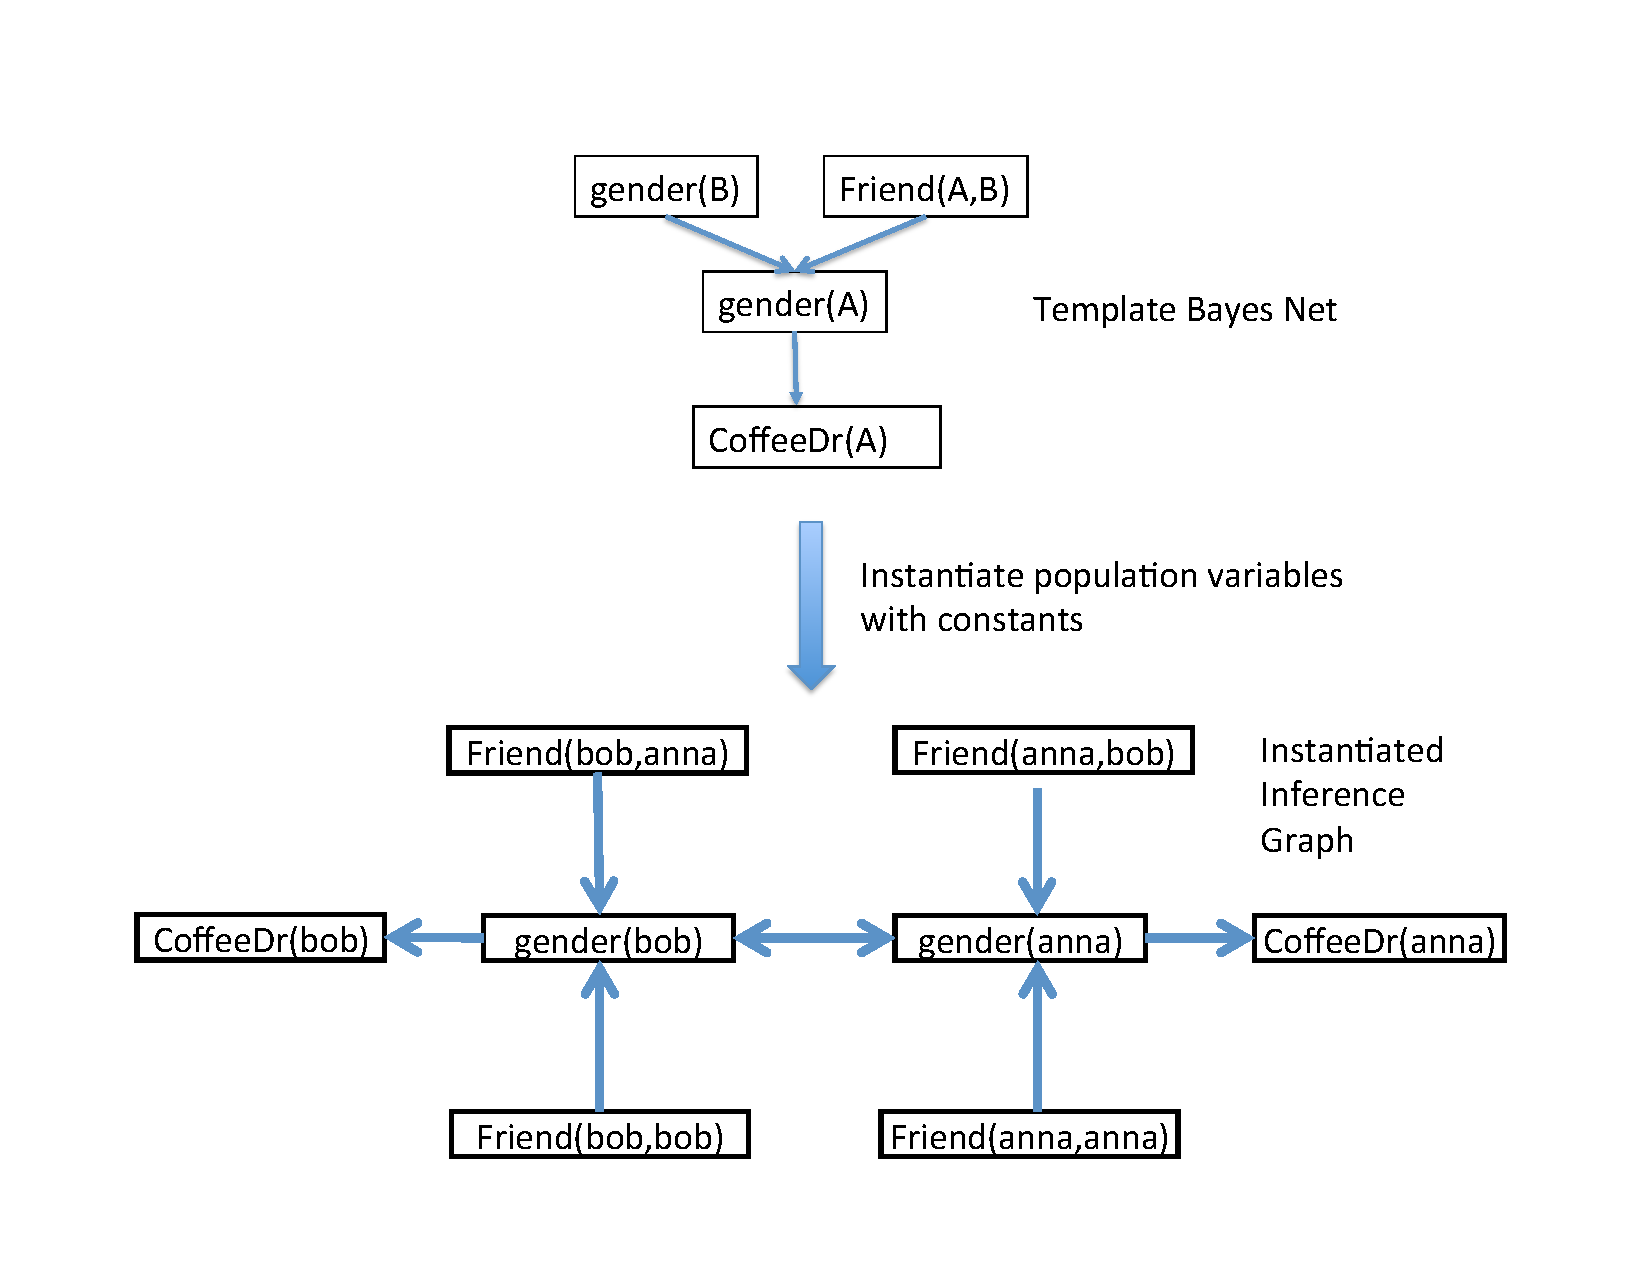
\includegraphics[width = 1 \textwidth]{figures/recurse-bn}
%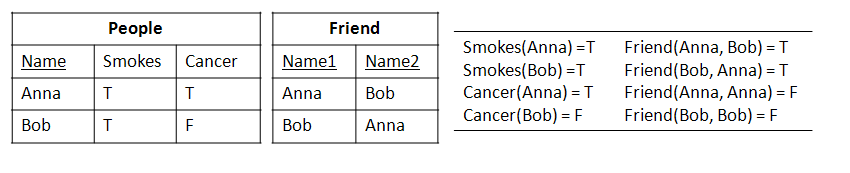
\includegraphics[width=1\textwidth]{database.png}
%}
\caption{A Bayes net template model (top) and the instantiated graph (bottom), with two individuals Anna and Bob in the domain of the first-order or population variables $\A,\B$. Population variables are to be instantiated with all constants that denote a member of the applicable set. 
 Cyclicity: The two instantiations $\A\gndlink anna,\B \gndlink bob$ and $\A\gndlink bob,\B\gndlink anna$ produce a cycle involving the two  edges $\it{gender}(anna) \rightarrow \it{gender}(bob)$ and $\it{gender}(bob) \rightarrow \it{gender}(anna)$. Imbalance: When predicting the value of $\it{gender}(anna)$, there is only one conditional probability factor associated with the instantiated child $\it{CoffeeDr}(anna)$, whereas there are many factors associated with the parents  $ \it{gender}(\B),\it{Friend}(\A,\B).$
\label{fig:recurse-bn}}
\end{center}
\end{figure}


%Multi-relational data are very common, from enterprise  databases to network data from the world-wide web and social media. 
%
%This paper presents a new log-linear multi-relational model for  Bayes nets, that has good predictive performance and permits highly scalable parameter learning. Log-linear models are a prominent model class that has been widely used in statistical-relational learning \cite{Sutton2007,Taskar2002,Domingos2009}. 
   %
\subsection{Gibbs Conditional Probabilities for relational data}  We base our model on a fundamental quantity for inference in generative models, the conditional probability of a random variable given an assignment of values to {\em all} remaining random variables. We call these probabilities fundamental because they are sufficient to compute a full joint probability distribution over all random variables via Gibbs sampling~\cite{Heckerman2000,Natarajan2012,Lowd2012}.
We therefore refer to them as \defterm{Gibbs conditional probabilities}, or simply Gibbs probabilities, distinguishing them from the conditional probability parameters of a Bayes net.\footnote{In the terminology of dependency networks \cite{Heckerman2000},  Gibbs  probabilities are referred to as local probability distributions. The WinBUGS system refers to them as full conditional probabilities~\cite{Lunn2000}.} In this paper we present a method for computing Gibbs probabilities for a Bayes net template model. 
%From these probabilities, any joint probability can be computed using Gibbs sampling. OS: already said.


For \iid{} data, a Bayes net is usually viewed as defining a joint probability distribution over assignments of values to its nodes, via the standard product formula \cite{Pearl1988}. The product formula entails that a Gibbs probability can be computed by a log-linear equation~\cite[Ch.14.5.2]{Russell2010}, which we refer to as the Bayes net Gibbs probability equation.
It is natural to also define Gibbs probabilities in log-linear form for the more general relational case where the BN is viewed as a template. 

A discriminative log-linear equation models a conditional probability for a target node value, given an assignment of values to other variables, called the input variables. In the case of a Gibbs probability, the input variables comprise all variables other than the target node. A log-linear model requires defining a set of features, and for each feature a feature function that returns a number for that feature and a given conditional probability to be computed \cite{Sutton2007}. The parameters of the model are feature weights, one for each feature. The conditional probability of the target node value given values for the input variables is proportional to the exponentiated weighted sum of the feature functions. In our proposed model, the set of features is the set of joint value assignments to a child and its parents in the BN structure. For each feature, the feature function is the frequency with which it is instantiated in the given query (i.e., its frequency given the conjunction of input variable values and the target node value). The frequencies need to be normalized with respect to the set of relevant features only, see Section~\ref{sec:predictors}.  The weight associated with a child-parent feature is computed as the log-difference of two quantities determined by the BN parameters: (i) the conditional probability of the child value, given its parent configuration, and (ii) the marginal probability of the child value. This weight measures the extent to which information about the parents changes the prior probability of the child value. We refer to the resulting log-linear equation as the \defterm{log-difference frequency equation}. The log-difference frequency equation reduces to the BN Gibbs probability equation in the case where the instantiation frequencies are either 0 or 1, that is, when the input variables determine a unique value for each node. 



To illustrate, suppose we wish to compute the probability that individual $\A = \it{sam}$ is male, using the template BN of Figure~\ref{fig:pbn}~(b). The input variables specify whether Sam is a coffee drinker, which other persons are his friends, and the gender of other people. There are two parents of the gender node in this template model. One feature in the log-linear model assigns these parents the values $\it{Friend}(\A,\B) = \true$ and $\it{gender}(\B) = \Man$. The feature function returns the percentange of Sam's friends that are male, given the values specified in the input variables. The weight associated with this feature is the log-ratio of two quantities: (i) the conditional probability that $\it{gender}(\A) = \Man$, given the assignment of values to its parents, which is specified as .63 in the BN. (ii) The BN marginal or unconditional probability that $\it{gender}(\A) = \Man$, which can be computed via BN inference as .55. So the weight of this feature is $w = ln(0.63/0.55) \approx 0.136$. The positive weight indicates that according to the BN template model, having a male friend raises the probability of being male.
%(e.g., the base rate of males in the user population).

\begin{figure}[htbp]
\begin{center}
\resizebox{1\textwidth}{!}{
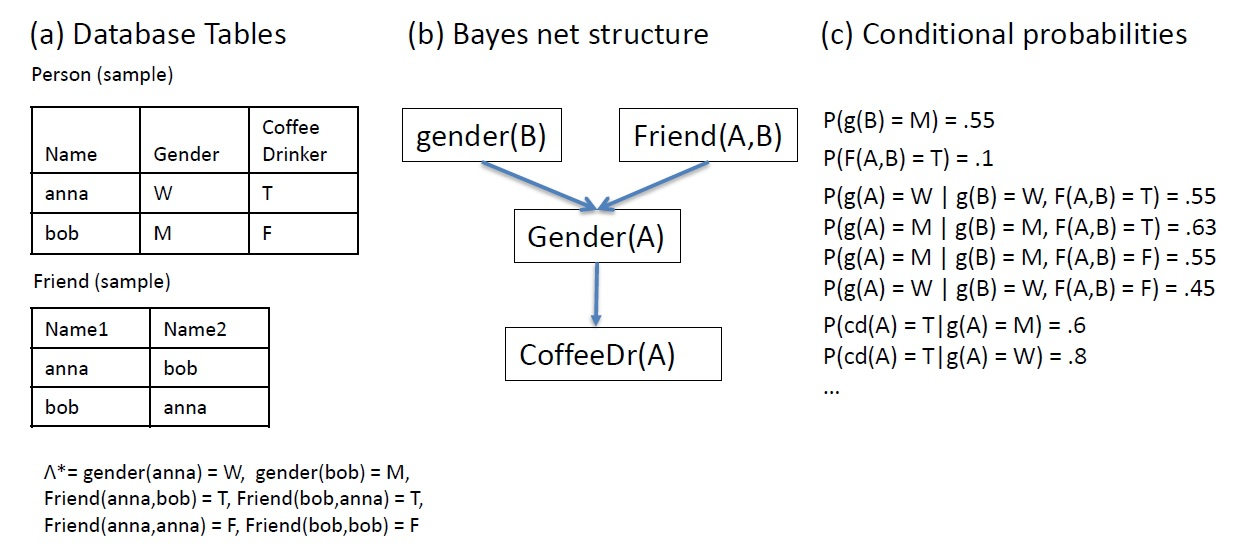
\includegraphics[width=1\textwidth]{pbn}
%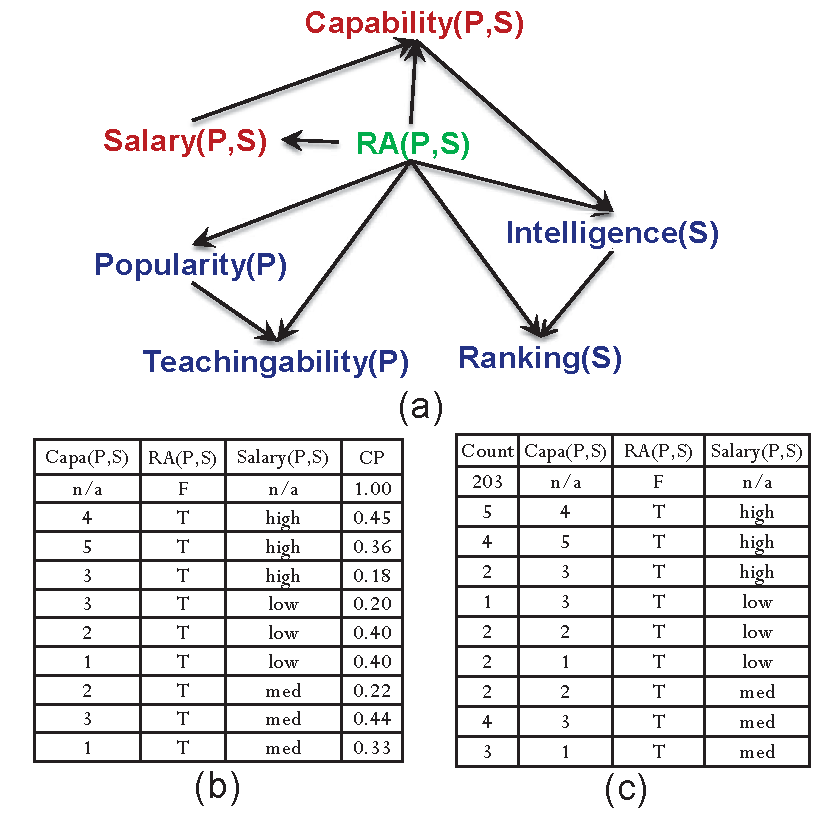
\includegraphics{figures/pbn.pdf}
}
\caption{Constructing a template Bayes net. (a) A relational database. By convention, a pair not listed in the Friend table are not friends. The $\it{Friend}$ relation represented by the Friend table is symmetric, $\it{Friend}(\A,\B) = \it{Friend}(\B,\A)$, and irreflexive,
$\it{Friend}(\A, \A) = \false$.
Only a subset of the rows are shown. 
(b) A Bayes net structure $G$ learned from the all the rows of the database.
%$\it{Friend}(\A,\B)$ is a relationship node, while the other three are attribute nodes. 
(c) The conditional probabilities $\bs{\theta}_G$ for $G$. There are slightly more men than women, there is a weak correlation between the gender of a person and that of their friends, and a woman is more likely to be a coffee drinker. 
}
\label{fig:pbn}
\end{center}
\end{figure}


This generalization of the standard log-linear BN Gibbs probability equation has theoretical justification as well. We prove that, under mild assumptions, the log-difference frequency equation can be viewed as a random instantiation extension of the BN equation: The log-difference value is equivalent to the expected value of choosing a random instantiation of the nodes in the template BN and applying the BN equation to this instantiation.

\subsection{Motivation}
%\point{Motivation}

The log-difference frequency equation has several advantages over previous inference methods for relational data.

\point{(1)~Interpretability} Log-linear weights learned using general optimization methods can be difficult to interpret, as they may reflect complex interactions between different correlated predictor variables. In contrast, a Bayes net parameter can be interpreted as a conditional probability, and reflects local statistics restricted to a parent-child configuration. Under the maximum likelihood criterion, the conditional probabilities can be interpreted in terms of empirical frequencies observed in a relational structure.

The log-difference transformation allows weights to be interpreted as usual in a log-linear model: a positive weight indicates positive relevance (the parent values raise the probability of a child value), a negative weight as negative relevance (parent values lower the child value probability), and a zero weight as irrelevance. 

\point{(2)~Scalability} 
Frequency estimates can be viewed as a type of \defterm{lifted learning} \cite{Schulte2012}, the approach of using only the sufficient statistics for a dataset rather than an iteration over ground facts. The computational cost of lifted learning scales well in both data size and the number of parameters in the model.


\point{(3)~Balancing Predictor Scales} A common choice of feature function is to use instantiation counts rather than frequencies. 
%As we discuss below, instantiation counts result from performing inference in an instantiated model, as in knowledge-based model construction. 
Whereas in the case of \iid{} data, counts and frequencies differ only by a constant population size factor, in relational data there is no such simple one-to-one relationship. For instance Sam and Morgan may each have 10 male friends, but if Sam has 10 friends in total and Morgan has 100 friends in total, the frequency of male friends for Sam is 100\%, whereas for Morgan it is only 10\%. In relational data, normalization involves {\em local} scaling factors (10 for Sam, 100 for Morgan), whereas in i.i.d. data it involves a single glocal factor (the sample size). It is intuitively clear that the count of male friends should be treated very differently in inferences for Sam than in inferences for Morgan. The general problem with using feature counts is that in a log-linear model with counts, features with more instantiations carry exponentially more weight. Count models tacitly conflate number of instantiations with degree of information.
In contrast frequency feature functions are on the common scale [0,1].
%
We refer to the diverging scale of feature counts as the \defterm{imbalance problem}. 

\subsection{Evaluation.} Using five standard databases, we evaluate the predictive accuracy obtained from log-difference frequency regression. We compare predictive performance with different choices of feature functions (counts vs. frequencies), and different choices of weights, including optimizing weights using general log-linear learning methods. We find that our log-linear model performs competitively with %existing 
alternative methods and is far faster than general weight learning. Our experiments provide evidence that because of the imbalance problem, maximum likelihoods do not lead to accurate predictions when they are used with feature counts.

\subsection{Comparison to Knowledge-Based Model Construction} \label{sec:kbmc} We contrast our approach at a high level with the traditional knowledge-based model construction approach. Section~\ref{sec:related} below provides a detailed discussion of previous work. In the KBMC approach, a template BN is instantiated to produce a {\em single instantiated BN}, called the inference graph by Neville and Jensen \cite{Neville2007}; see Figure~\ref{fig:recurse-bn}. The standard Bayes net product formula can be applied in the instantiated model to assign joint probabilities for all instantiated nodes. In the relational case, this provides a method for computing, from a template BN, a joint probability for each collection of facts about individuals and their relationships~\cite{Getoor2007c,Kersting2007}. An advantage of our approach is that it avoids several challenges for KBMC. 

\point{(1) Multiple Parents and Scalability} In the instantiated model, a parent configuration is usually instantiated multiple times for a given child node. This ``multiple-parent problem'' \cite{Natarajan2008} requires merging the information from different parents into a single conditional probability for a child node given a specification of values for the multiple parents. Two common approaches are using (i) combining rules \cite{Kersting2007} and (ii) aggregation functions \cite{Getoor2007c}. Adding combining rules or aggregation functions leads to very rich and expressive models. The resulting likelihood function does not factor as a product, unlike the BN likelihood function in the nonrelational case, and therefore optimizing it requires local search methods rather than using empirical frequency estimates  \cite{Kersting2007,Natarajan2009}. Also, it may be necessary to learn which combining rules/aggregate functions are best for a given dataset, which increases the learning complexity further.


\point{(2)~The Cyclicity Problem} Cyclicity arises because the instantiated Bayes net may contain cycles even if the template Bayes net does not.
This occurs in the common case that a dataset features auto-correlations, where the value of an attribute for an individual depends on the values of the same attribute for related individuals \cite{Neville2007,Schulte2012a}. Figure~\ref{fig:recurse-bn}  provides an example.
In the presence of cycles, the instantiated model is not a valid Bayes net structure (which must be acyclic).
%usual Bayes net product formula does not define probabilistic inferences.
This has been a knotty problem for defining a joint distribution using a template semantics~\cite{Domingos2007,Taskar2002,Getoor2007c}. Since a Gibbs conditional equation defines a local distribution that pertains to a single instantiated node, not a full instantiated graph, it is well-defined even when the full instantiated graph contains cyclic dependencies.

\point{(3)~The imbalance problem} A joint probability distribution entails conditional probabilities. We can therefore compare the Gibbs probabilities that are entailed by an instantiated model with the Gibbs probabilities defined by our proposed log-linear model.
As noted above, the product formula for the joint probability of a Bayes net model entails that that the Gibbs conditional probability has a log-linear form corresponding to a product of conditional probabilities. In the instantiated model, there is one such conditional probability for each instantiation of a parent-child configuration. This means that {\em in the instantiated model, the feature function is the instantiation count}. For example, consider the template structure $\it{intelligence}(S) \rightarrow \it{difficulty}(C) \leftarrow \it{Registered}(S,C)$. This represents a correlation between the difficulty of a course and the intelligence of students who take the course. If our target node value is $\it{intelligence}(sam) = hi$, the prediction will be based on a product of conditional probabilities of the form $\prod_{c}P(\it{difficulty}(c)|\it{intelligence}(sam) = hi)$, one for each course $c$ that Sam is registered in. 
Notice that the product of conditional probabilities arises regardless of what combining rule or aggregation function is specified for the parents of an instantiated node.
%, because the Gibbs probability for a target is derived from a product that includes one term for the conditional probability of {\em each} of the target's instantiated children. 
Therefore using the standard BN product formula with a single instantiated inference model entails a ``ground-and-count'' log-linear model, and suffers from the imbalance problem.  The imbalance problem also arises for other graphical model classes that use the KBMC approach with a factored joint probability function, such as undirected Markov net models~\cite{Domingos2009,Taskar2002}. 





\strongpoint{Contributions and Significance} Our main contributions are: 
%\item An empirical evaluation of log-linear Bayes net models with count predictors, together with an analytic solution for the likelihood maxima.
\begin{enumerate}
\item An approach to relational Bayes net inference that applies a template semantics to Gibbs conditional probabilities on a local region of an instantiated Bayes net, rather than the entire net.
\item A new log-linear equation that computes, given a template Bayes net, a Gibbs conditional distribution for making inferences about relational data. The new log-linear model performs well with easily computed maximum likelihood estimates for the Bayes net parameters (observed conditional frequencies).

\end{enumerate}

Standardizing the scale of variables is a common preprocessing steps in building linear models \cite{Bishop2006}. It may therefore seem unsurprising that normalizing counts improves statistical-relational predictions. Nonetheless, we believe that the innovation of replacing counts by frequencies as the feature function has important consequences, both conceptual and practical.  

(1) As we discussed, the most common KBMC approach of defining inferences with respect to a single instantiated inference model implicitly entails using counts as feature functions. In contrast, using frequencies as feature functions is  consistent with a random selection interpretation of the Bayes net model, where population variables represent a random draw from the associated population. The random selection interpretation was developed in detail by Halpern \cite{Halpern90} and Bacchus \cite{Bacchus90} in their classic work on first-order probability logic. Adapting the random selection interpretation for first-order Bayes net models is a recent development in statistical-relational learning \cite{Schulte2013}. Thus the difference between counts and frequencies mirrors an alternative in the semantics of a first-order Bayes net. 

(2) The instantiation frequencies of Bayes net node assignments, which we propose to use for computing Bayes net parameters, can be interpreted in terms of {\em class-level probabilities} \cite{Schulte2013} (also called type 1 probabilities \cite{Halpern90}). For instance, the frequency of the condition $\it{gender}(\A) = \Woman$ represents the proportion of women in the class of persons. The inference models that we develop in this paper, define {\em instance-level probabilities} for the attributes of specific individuals (also called type 2 probabilities \cite{Halpern90}). For instance, our log-linear equation computes a value for the probability that $\it{gender}(sam) = \Woman$, conditional on known facts about $sam$, where $sam$ denotes a particular individual. The log-linear equation we propose in this paper therefore computes instance-level probabilities---for the target node values---from given class-level probabilities---the Bayes net parameters. The question of how to compute instance-level probabilities from class-level statistics has received considerable attention from leading AI researchers \cite{Bacchus1992,Halpern2006}. Our log-linear model represents a new approach to this long-standing question.



(3) Current relational regression models have difficulty scaling to medium-sized datasets, especially those with many descriptive attributes \cite{Khot2011,Schulte2011,Natarajan2012}. Our work extends the practical applicability of relational learning to such datasets, and provides a strong scalable baseline learning method.

\strongpoint{Paper Organization}
We begin (Section~\ref{sec:background}) with background and define the notation for relational Bayes net models.
%, in terms of random selection and ground graphical models. 
% and shows that conditional probabilities maximize the unnormalized likelihood. We then present the frequency regression model. 
Section~\ref{sec:theequation} presents the new log-linear relational regression model, which we compare
with alternative formulations in Section~\ref{sec:alternatives} and then evaluate
on five benchmark databases in Sections~\ref{sec:empirical-comparison} and~\ref{sec:general-weights}.
%In Section~\ref{sec:mln-boost} we use the same databases to compare our approach to MLN-Boost \cite{Khot2011}.
Section~\ref{sec:random}  shows the theoretical equivalence between the frequency regression value and a random instantiation semantics.
%In Section~\ref{sec:comparison} we establish the theoretical equivalence of frequency reqression with equations for Markov networks and dependency networks. 
We end with related work in Section~\ref{sec:related}, and conclude with suggestions for future work in Section~\ref{sec:conclusion}.

 
\section{Background: Bayes Nets for Relational Data} \label{sec:background} We adopt function-based notation from logic for combining Bayes nets with relational concepts \cite{Russell2010,Poole2003,Getoor2006,Chiang2012}. Different communities in statistics and logic use different terms for similar concepts, and similar terms for different concepts. We strive for notation that is as broadly accessible as possible. Table~\ref{table:relational-notation} summarizes our notation for relational concepts. %, and note conflicts of terminology when we cannot avoid them. 


\begin{table}[htbp]
\vspace{-0.4cm}
\caption{Summary of Notation for Relational Concepts}
\begin{tabular}{lp{8cm}p{5cm}}\label{table:relational-notation}
Notation & Explanation & Example \\\hline
$\A,\B$ & \defterm{Population Variables} & $\A$\\
$\TT, \UT, \VT$ & \defterm{Terms}. A term consists of a \defterm{functor} and its arguments.  The arguments may be any combination of 
\defterm{population variables} and \defterm{constants}. & $\it{gender}(\A)$ \\
$\TF, \UF, \VF $ & \defterm{Term Tuples}.  A list of terms. A given term can occur at most once. Order is significant. & $\it{gender}(\B); \it{Friend}(\A,\B)$\\ $\Range{\TT}, \Range{\TF}$ & The \defterm{range of a term} and the \defterm{range of a term tuple}. The range of a \defterm{term} is the range of its functor. The range of a tuple is the Cartesian product of the ranges of the constituent \defterm{terms}.& $\Range{\it{gender}(\B), \it{Friend}(\A,\B)} = \{\Woman,\Man\} \times \{\true,\false\}$ \\
$\TV, \UV, \VV$ & \defterm{Values} from the ranges of $\TT, \UT, \VT$. & $\Man;\true$ \\
$\TTuple, \UTuple, \VTuple$ & \defterm{Tuples of values} from the ranges of $\TF, \UF, \VF$. & $(\Man,\true)$ \\
%$\Vars{\TT}, \Vars{\TF}$ & The \defterm{variables of a term} and the \defterm{variables of a vector}. A list of all the %unique 
%population variables in a term or vector. & $\Vars{\it{Friend}(\A,\B)} = \{\A,\B\}.$ \\
$\TT = \TV$ & \defterm{Literal}. A term bound to a value from its range. 
& $\it{Friend}(\A,\B) = \true$ \\
$\TF = \TTuple$ & \defterm{Literal conjunction}. A conjunction bound to a tuple of values from its \defterm{range}. Every \defterm{term} in a literal conjunction is bound to its corresponding value. & $\it{Friend}(\A,\B) = \true$,$\it{gender}(\A)=\Woman$\\
%A single \defterm{grounding} may be applied to all terms in the conjunction. \\
$\grounding$ %, $\{\A_{i}\gndlink\a_{1},\ldots,\A_{j}\gndlink \a_{j}\}$ 
& \defterm{Instantiation}.
%$\grounding: \TF \rightarrow \PG{\TF}$ & \defterm{Grounding}. 
An instantiation maps zero or more \defterm{population variables} to appropriate \defterm{constants}.  & $\grounding = \{\A\gndlink anna,\B\gndlink bob\}$
%We will typically assume groundings, implying them in the $\PG{\TF}$ and $\FG{\TF}$ notations. 
 \\
$\FG{\TT}, \FG{\TF}$ & \defterm{Fully ground term/tuple}. All arguments to all functors are constants. Equivalently, the term/tuple does not contain any population variables. & $\it{gender}(anna),\it{Friend}(anna,bob)$ \\
$\DB$ & %\defterm{Database}. A 
Complete \defterm{literal conjunction} comprising \defterm{fully grounded} terms.
The conjunction binds {\em every} ground term to a value. & See Table~\ref{table:count-examples}.
%$\it{gender}(anna) = W$, $\it{gender}(bob) = M,$ $\it{Friend}(anna,bob) = \true,$ $\it{Friend}(bob,anna) = \true,$ $\it{Friend}(anna,anna) = \false,$ $\it{Friend}(bob,bob) = \false$
%For \defterm{literal terms} whose \defterm{ranges} are boolean, we assume that any fully ground instance absent from the database has the value $\false$. For a given computation of \defterm{Gibbs conditional probability}, the database is fixed and does not contain the term for which the probability is being computed. 
\\
$\Count{\TF = \TTuple}{\DB}$ & \defterm{Instantiation Count.}  Counts the number of groundings of $\TF = \TTuple$ that evaluate as true in $\DB$. A \defterm{grounding} instantiates {\em all} population variables in $\TF$.  & 
%$\Count{\it{gender}(\A) = \Woman, \it{Friend}(\A,\B) = \true}{\DB}$ = 1. 
See Table~\ref{table:count-examples}.\\
\end{tabular}
\end{table}


\subsection{Relational Concepts.} A  \defterm{population} $\population$ is a set of individuals. Individuals are denoted by lower case identifiers (e.g., $\it{sam}$). Identifiers representing individuals are called \defterm{constants}. 

\subsubsection{Functor Notation}
A \defterm{functor}
$
\functor: \population_{1},\ldots,\population_{a} \rightarrow \outdomain_{\functor}
$
maps a list of individuals to a functor value, 
where $\outdomain_{\functor}$ is the output type or \defterm{range} of the functor. In this paper we consider only functors with a finite range.
%, disjoint from all populations.  
If $\outdomain_{\functor} = \{\true,\false\}$, the functor $\functor$ is a (Boolean) \defterm{predicate}; other functors are called \defterm{attributes}. A predicate with more than one argument is called a \defterm{relationship}. Predicates typically represent the presence of a binary property or a relationship, while attributes typically represent properties that can take multiple values. 
%The finite-ranged attributes considered in this paper are syntactic sugar: they could be systematically replaced by sets of unary predicates, such as replacing $\it{gender}$ with $\it{Man}$ and $\it{Woman}$. 
% OS: this would change the learning behaviour, see Domingos and our AAAI paper.
We use lowercase for attribute functors and uppercase for predicates.
We define two kinds of variables, with distinct domains: (i) A \defterm{population variable} varies over a population domain. The same population may be associated with more than one population variable. We use an outline Latin font for population variable ($\A,\B,\ldots$).
%We index population variables if more than one is associated with the same population (e.g., $\A, \B, \it{Student}$). 
(ii) A \defterm{term}
is an expression of the form $\functor(\terms) \equiv \functor(\term_{1},\ldots,\term_{k})$, where 
each $\term_{i}$ is a population variable or a constant of the appropriate argument type for that functor.\footnote{The traditional term in first-order logic for a term variable is ``function term''. In statistical-relational learning, alternative terms include ``parametrized random variable'' \cite{Poole2003}, ``atom'' \cite{Chiang2012}, ``Bayesian atom''  \cite{Kersting2007}, and ``functor random variable'' \cite{Schulte2012}.} A term can be assigned values in the range of its functor.

In a context where the functor and arguments of terms are not important, we denote them by uppercase Latin letters ($\TT,\UT,\ldots$).

A \defterm{literal} is an assignment to a term, denoted generically as $\TT = \TV$, where $\TV$ is in the range of the functor for $\TT$. 
% where $v$ is in the range of $\functor$ and $\functor(\term_{1},\ldots,\term_{a})$ is a PRV. 
Literals can be combined to generate \defterm{formulas}. 
In this paper we consider only formulas that are \defterm{conjunctions} of literals, denoted by the Prolog-style comma notation, e.g., 
%$\functor(\term_{1},\ldots,\term_{a}) = v, \ldots,\functor_{z}(\term'_{1},\ldots,\term'_{a'}) = v'$. The corresponding more compact notation for a conjunctive formula would be 
$\TT = \TV, \ldots, \UT = \UV$, for which we also use the  vector notation $\TF = \TTuple$.


\subsubsection{Groundings and Relational Structures}
An term is \defterm{ground} if it contains no population variables. We mark fully ground terms and formulas by an asterisk, $\FG{\TT}$. An \defterm{instantiation}  for a term assigns a constant to a set of the population variables in the term. Formally, an instantiation $\gamma$ is a set $\{\A_{i}\gndlink\a_{1},\ldots,\A_{j}\gndlink \a_{j}\}$ 
that assigns a constant $\gamma(\A_{i})$ to each variable $\A_{i}$ from its population. The expression $\Ground{\TT}$ denotes the term that results from applying the substituition $\gamma$ to all variables in $\TT$. If the instantiation $\gamma$ specifies a constant for all the population variables that occur in the term, the resulting term is ground, and $\gamma$ is called a \defterm{grounding}. An instantiation is applied to a formula by applying it to all terms in the formula. Thus a grounding of a formula is an instantiation that grounds of all its terms.


A \defterm{relational structure} is a (model, interpretation) pair that assigns a unique value to each ground term \cite{Chiang2012}. Assuming a finite list of functors, and that all populations are finite, a relational structure is equivalent to a \defterm{complete conjunction} of ground literals $\DB \equiv (\FG{\TF} = \TTuple)$. The ground literals in the relational structure are called \defterm{facts}. A conjunction of ground literals evaluates as true in a relational structure if each of its conjuncts is a fact. A well-studied operation~\cite{Schulte2013} for statistical learning is to count, for a given nonground formula $\TF = \TTuple$ and complete conjunction $\DB$, the number of groundings of the formula that evaluate as true in the complete conjunction. Note that only groundings that instantiate exactly the population variables that appear in $\TF$. We refer to this quantity as the formula's \defterm{instantiation count}, denoted by $$\Count{\TF = \TTuple}{\DB}.$$

\subsubsection{Examples.}

Figure~\ref{fig:pbn}(a) shows the facts in a relational structure, represented as database tables. For this example only, let us assume that the tables represent a relational structure completely, and hence specifies a complete conjunction $\DB$. Table~\ref{table:count-examples} shows examples of instantiation counts for this complete conjunction.

\begin{table}[htdp]
\caption{Instantiation counts in the database of Figure~\ref{fig:pbn}. For the sake of the example, we treat the database as specifying a complete conjunction $\DB =$  $\{gender(anna) = W$,  $gender(bob) = M$, $Friend(anna,bob) = T$, $Friend(bob,anna) = T$, $Friend(anna,anna) = F$, $Friend(bob,bob) = F
\}$.}
\begin{center}
\begin{tabular}{lc}
Formula & Instantiation Count\\\hline
$\it{gender}(\A) = \Man$ & 1 \\
$\it{Friend}(\A,\B) = \true$ & 2\\
$\it{Friend}(bob,\B) = \true$ & 1 \\
$\it{gender}(\B) = \Man, \it{Friend}(\A,\B) = \true$ & 1 \\
$\it{gender}(anna) = \Man, \it{Friend}(\A, anna) = \true$ & 0
\end{tabular}
\end{center}
\label{table:count-examples}
\end{table}%


\begin{table}
\vspace{-1cm}
\caption{Summary of Notation for Template Bayes Nets}
\begin{tabular}{lp{8cm}p{4cm}}\label{table:BN-notation}
Notation & Explanation & Example  \\\hline
$\Pa{\TT}: \TT \rightarrow \TF$ & \defterm{Parents}. The \defterm{terms} associated with the parent nodes of the unique Bayes net node associated with $\TT$. The parent terms will be distinct. & $\Pa{\it{gender}(\A)}$ = $\langle\it{gender}(\B),\it{Friend}(\A,\B)\rangle$
%Any \defterm{grounding} applied to $\TT$ will also be applied to $\TF$. 
\\
$\Ch{\TT}: \TT \rightarrow \TF$ & \defterm{Children}. The \defterm{terms} associated with the child nodes of the unique Bayes net node associated with $\TT$. 
& $\Ch{\it{gender}(\A)}$ = $\it{CoffeeDr}(\A)$
%Any \defterm{grounding} applied to $\TT$ will also be applied to $\TF$.
\\
%$\Mrange{\TT}$ & \defterm{Value in the Markov range}. Tuple of values from $\Range{\MB{\TT}}$. \\
$\Prange{\TT}$ & \defterm{Value in the parent range}. Tuple of values from $\Range{\Pa{\TT}}$. & $\langle \Man,\true \rangle$\\
%$\jprob{\TF = \TTuple[0.6ex]}$ & \defterm{Joint probability} of a literal conjunction. \\
$\TT=\TV,\Pa{\TT} = \Prange{\TT}$ & \defterm{Family Configuration} that specifies values for node $\TT$ and its parent nodes $\Pa{\TT}$. & $\it{gender}(\A) = \Man,$ $\it{gender}(\B) = \Woman,$ $\it{Friend}(\A,\B) = \true$\\
$\cprob{\TT = \TV}{\Pa{\TT} = \Prange{\TT}}$ & \defterm{Conditional probability} of a node value given a parent configuration. & $\cprob{\it{gender}(\A) = \Woman}{\it{gender}(\B) = \Woman,\it{Friend}(\A,\B) = \true}$ = $0.55$
\\
%$\cprob{\TT = \TV}{\UF = \UTuple}$ & \defterm{Conditional probability} of a literal term given a literal conjunction.  \\
$\jprob{\TT = \TV}$ & \defterm{Marginal probability} of a node value entailed by the Bayes net. & $P(\it{gender}(\A)= \Man)$ = $0.55$
\end{tabular}
\end{table}


\subsection{Bayes Nets for Relational Data.} \label{sec:graph-relational}




A Bayes net (BN) is a pair
$\langle{G,\bs{\theta}_G}\rangle$, where $G$ is a directed acyclic graph and $\bs{\theta}_G$ is a set of parameters that specify the  probability distributions of children conditional on instantiations of their parents. A \defterm{Template Bayes Net} (TBN) is a Bayes net whose nodes are nonground terms~\cite{Poole2003,Schulte2011}. That is, every node in the Bayes net is a term containing one or more population variables. When describing Bayes nets, we use ``term'' and ``node'' interchangeably. Table~\ref{table:BN-notation} summarizes our notation for Bayes nets and Figure~\ref{fig:pbn}(b) shows an example net.

A \defterm{family} comprises a node and its parents. A \defterm{family configuration} specifies a value for a child node and each of its parents. Since we consider functors with discrete ranges only, there are only finitely many family configurations. Using the notation in Table~\ref{table:BN-notation}, a family configuration is equivalent to the conjunction $\TT=\TV,\Pa{\TT} = \Prange{\TT}$. For each family configuration, a \defterm{Bayes net parameter} $$\cprob{\TT = \TV}{\Pa{\TT} = \Prange{\TT}}$$ specifies the probability of the child value $\TV$ given the parent values $\Prange{\TT}$.\footnote{For \iid{} data, a commonly  used notation for a BN parameter is $\theta_{ijk}$~\cite{Heckerman1998}.} Given a complete conjunction $\DB$, the number of family configurations is\footnote{For \iid{} data, a commonly  used notation for this quantity is $\instances_{ijk}$~\cite{Heckerman1998}.} $$\Count{\TT=\TV,\Pa{\TT} = \Prange{\TT}}{\DB}.$$

The parameter values for a Bayes net define a joint distribution over its nodes via the standard product formula. A parametrization therefore entails a marginal, or unconditional, probability for a single node. We denote the marginal probability that node $\TT$ has value $\TV$ by the notation

$$\jprob{\TT = \TV}.$$


\subsection{Bayes Net Gibbs Probabilities.}

We review the equation for Gibbs conditional probabilities for a Bayes net that specifies a joint distribution over its nodes via the standard product formula \cite{Pearl1988}. 
Inferring a Gibbs conditional probability can be represented as a probabilistic query
$$\Gprob{\TT = \TV} {\VF = \VTuple} = ?$$
\noindent where $\TT$ is the target node, $\TV$ is a value for the target node, and $\VTuple = \VF$ specifies a value for every other node. The product formula for the Bayes net joint distribution entails that the Gibbs probability is proportional to a product of conditional probabilities for the target node and its children~\cite[Ch.14.5.2]{Russell2010}:  
\begin{equation} \label{eq:bn-mb-product}
\Gprob{\TT = \TV} {\VF = \VTuple} \propto \prod_{\UT \in \{\TT\} \cup \Ch{\TT}} \cprob{\UT = \UV}{\Pa{\UT} = \Prange{\UT}}
\end{equation}
where $\UV$ and $\Prange{\UT}$ are specified by the values in $\TV,\VTuple$ for the corresponding nodes. The product is a number between 0 and 1 that needs to be normalized to obtain the Gibbs conditional probability.

\strongpoint{Example} For the Bayes net of Figure~\ref{fig:pbn}, consider the query

$$\Gprob{\it{gender}(\A) = \Woman} {\it{gender}(\B) = \Woman, \it{Friend}(\A,\B) = \true, \it{CoffeeDr}(\A) = \true}.$$

\noindent By Equation~\ref{eq:bn-mb-product}, this probability is proportional to 

\begin{eqnarray*}
\cprob{\it{gender}(\A) = \Woman}{\it{gender}(\B) = \Woman, \it{Friend}(\A,\B) = \true} & \cdot & \cprob{\it{CoffeeDr}(\A) = \true}{\it{gender}(\A) = \Woman} \\
= 0.55 &\cdot &0.8 = 0.44.
\end{eqnarray*}


\subsection{Log-Linear Models}

Equation~\ref{eq:bn-mb-product} can be seen as an instance of a standard log-linear schema as follows. The general equation form that defines a \textbf{discriminative log-linear model} \cite[Sec.4.2.2.1]{Sutton2007} is 

\begin{equation} \label{eq:log-linear}
\Gprob{\TT = \TV} {\VF = \VTuple} \propto exp(w_{\TV} + \sum_{i=1}^{K} w_{i} f_{i}(\TV,\VF)),
\end{equation}

\noindent where $\TT$ is the target or output variable, and $\VTuple = \VF$ represents an assignment of values to the input variables. The model is based on a finite set of $K$ features, and for each feature there is a real-valued weight parameter $w_{i}$. The term $w_{\TV}$ is a bias weight that may depend on the target node value $\TV$ but not the input variables. The functions $f_{1},\ldots,f_{k}$ are \textbf{feature functions}, such that $f_{i}$ returns a real number for feature $i$ given values for both the target and input variables. A log-linear equation defines a log-linear model; we use the term ``equation'' to emphasize the mathematical form, and the term ``model'' to emphasize the parameter space.

Rewriting Equation~\ref{eq:bn-mb-product} as 

\begin{equation} \label{eq:bn-mb}
\Gprob{\TT = \TV} {\VF = \VTuple} \propto exp(\sum_{\UT \in \{\TT\} \cup \Ch{\TT}} \ln\cprob{\UT = \UV}{\Pa{\UT} = \Prange{\UT}})
\end{equation}

\noindent shows that a BN Gibbs probability follows a log-linear model with the following specifications. (1) The features are all family configurations whose child node is either the target node or a child of the target node. (2) The feature weights are the log-conditional probabilities associated with a family configuration; the bias weight is 0. (3) The feature function for each a family configuration returns 1 if the family configuration is specified by the conjunction $(\TV,\VTuple)$ of input and output variables, 0 otherwise. 

This log-linear equation specifies the Gibbs probability for the nonground terms/nodes in the template Bayes net. Our goal in this paper is to define inference for queries whose target are ground terms. We therefore want to generalize Equation~\eqref{eq:bn-mb} for ground terms. The log-linear equations for ground terms that we consider are also based on products of the Bayes net parameters, combined with transformations. 



\section{The Log-Difference Frequency Equation} 
\label{sec:theequation}

\begin{table}
\vspace{-1cm}
\caption{Summary of Notation for Relational Gibbs Probabilities}
\begin{tabular}{lp{4cm}p{4cm}}\label{table:equation-notation}
Notation & Explanation & Example \\\hline
$\FG{\Ground{\TI}}$ & Fully Ground Target Node & $[\it{gender}(\A)]_{\{\A\gndlink sam\}} = \it{gender}(sam) $ \\
$\TV$ & Target Node Value & $\Man$\\
$\QC$ & \defterm{Query Conjunction.} A fully ground literal conjunction that binds every term to a value except for the target node & See Table~\ref{table:count-examples}\\
$\Gprob{\FG{\Ground{\TI}} = \TV} {\QC}$ & \defterm{Gibbs conditional probability}, or a \defterm{Query} & $\Gprob{\it{gender}(sam) = \Man}{\QC}$ \\
$\Appendterm{\Ground{\UI}  = \UV} {\Ground{\Pa{\UI}} = \Prange{\UT}}$ & Partially ground query family configuration &  $\it{gender}(sam) = \Man,$ $\it{gender}(\B) = \Woman,$ $\it{Friend}(sam,\B) = \true$\\
$\Relcount{\Appendterm{\Ground{\UI}  = \UV} {\Ground{\Pa{\UI}} = \Prange{\UT}}} {\QC,\Ground{\TI} = \TV}$ & \defterm{Relevant Instantiation Count} of a query family configuration. & See Section~\ref{sec:predictors}. \\
$\Relfreq{\Appendterm{\Ground{\UI}  = \UV} {\Ground{\Pa{\UI}} = \Prange{\UT}}} {\QC,\Ground{\TI} = \TV}$ & \defterm{Relevant Instantiation Frequency} of a query family configuration. & See Section~\ref{sec:predictors}. \\


%$\RelcountC{\UT=\UV,\Pa{\UT} = \Prange{\UT}}{\QC,\Ground{\TI} = \TV}{\grounding}$ & \defterm{Constrained Count of Relevant Instantiations} of a query family configuration. & See the text. \\
%$\RelfreqC{\UT=\UV,\Pa{\UT} = \Prange{\UT}}{\QC,\Ground{\TI} = \TV}{\grounding}$ & \defterm{Constrained Frequency of Relevant Instantiations} of a query family configuration. & See the text. \\
%$\Relfreq{\TF}{\DB}$ & \defterm{Relevant frequency} of a \defterm{conjunction}, given a \defterm{database}. See the text for the definition of relevant frequency. \\& $\it{gender}(\A)$ \\
\end{tabular}
\end{table}


%In this section we generalize Equation~\ref{eq:bn-mb} to the relational case. 
We propose a log-linear equation for computing a Gibbs conditional probability in closed form, given (i) a ground target node (the output variable), (ii) a target value for the target node, (iii) a complete set of values for all ground terms other than the term of the target node (the input variables), and (iv) a template Bayes net. We refer to our proposal as the 
\defterm{log-difference frequency equation}. Our notation is summarized in Table~\ref{table:equation-notation}. For now we assume that component~(iv), the template BN, is fixed (Section~\ref{sec:predictors} discusses structure learning), and consider in this section components~(i)--(iii). 
%The features and weights can be computed in closed-form from the BN template, and the feature functions from the BN template and the given query. 
Figure~\ref{fig:bn-flow} shows the program flow for computing a Gibbs probability using the log-difference frequency equation.

% We begin with components~(i)--(iii) and introduce component~(iv), the template net, in Section~\ref{sec:predictors}.
% 

\begin{figure}[htbp]

\begin{center}
\vspace{-2.6cm}
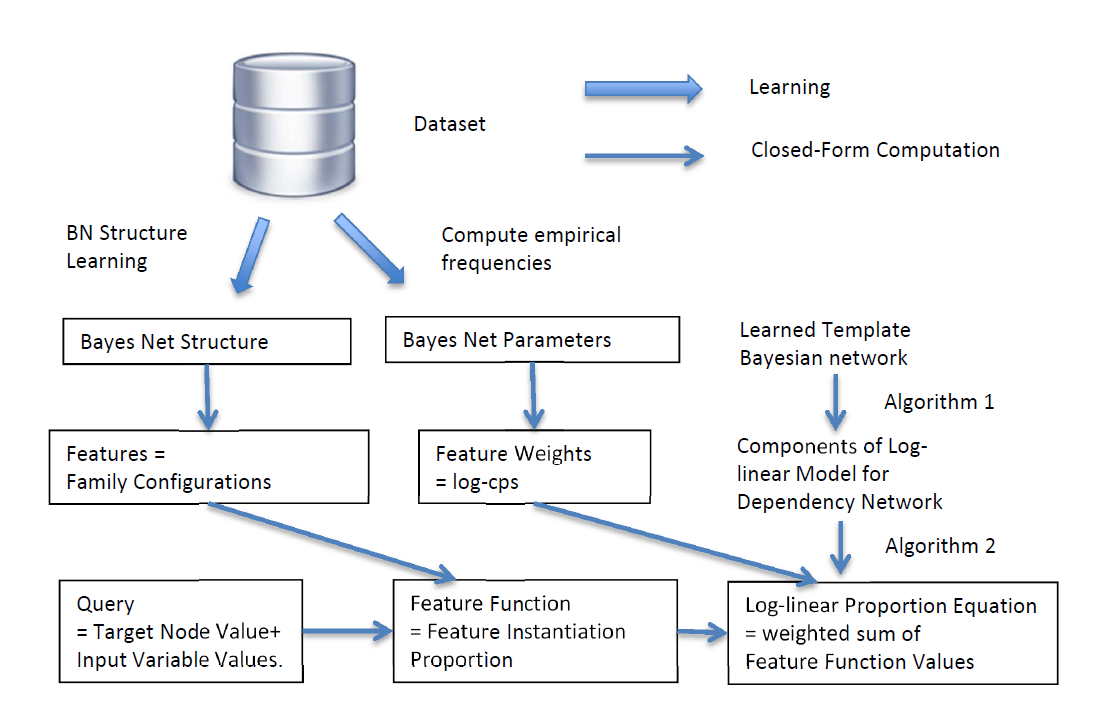
\includegraphics[width=0.7\textwidth]{figures/bn-regress}
\caption{The program flow for computing relational Gibbs probabilities with a template Bayes net. Features and weights are computed from the Bayes net. Feature function values are computed for each query.}
\label{fig:bn-flow}
\end{center}
\end{figure}


 \subsection{Conditional Queries} Conditional queries comprise the following elements:
 
\begin{enumerate}
\item A \defterm{target literal} $\FG{\Ground{\TI}} = \TV$, where $\FG{\Ground{\TI}}$ denotes a ground term that results from applying the grounding $\grounding$ to the term $\T$.
\item A conjunction $\DB$ that specifies a value for each ground term other than $\FG{\Ground{\TI}}$. The conjunction $(\Qconj)$ specifies the value of {\em every} ground term; we refer to it as the \defterm{query conjunction}.
\end{enumerate}

A Gibbs conditional probability corresponds to a probabilistic \defterm{query}

$$\Gprob{\FG{\Ground{\TI}} = \TV} {\DB} = ?$$

\noindent For example, a target node may be $\it{gender}(sam)$, which results from the grounding $\it{gender}(\A)\{\A\gndlink sam\}$.\footnote{The node $\it{gender}(sam)$ can also be defined by the grounding $\it{gender}(\B)\{\B\gndlink sam\}$. To make our definition unambiguous, we assume that the BN is in main functor format and that the template node $\T$ is the main functor node for its functor; see \cite{Schulte2012a}.}  The conjunction $\DB$ specifies a value for all ground terms other than $\it{gender}(sam)$.

\subsection{Features and Feature Weights} \label{sec:features} The features are all family configurations whose child node is either the target node or a child of the target node, as with nontemplate BNs. Thus the set of features equals the set of \defterm{query family configurations}

$$\QFC \equiv \{\Appendterm{\UI  = \UV} {\Pa{\UI} = \Prange{\UT}}: \UT \in \{\TT\} \cup \Ch{\TT}, \UV \in \Range{\UT}, \Prange{\UT} \in  \Range{\Pa{\UT}}\}.$$

The weights are computed as follows.

\begin{enumerate}
\item The offset weight $$w_{0} \equiv \ln \jprob{\TT = \TV}$$ is the log-marginal probability of the target node value, as entailed by the template Bayes net. (Apply the standard product formula for joint probabilities and sum over all joint probabilities where  $\TT = \TV$). 
\item For each query family configuration 
%$\Appendterm{\UI  = \UV} {\Pa{\UI} = \Prange{\UT}}$
%$$\UT = \UV,\Pa{\UT} = \Prange{\UT},$$ 
there is an associated weight $$w \equiv \left[ \ln \cprob{\UT = \UV}{\Pa{\UT} = \Prange{\UT}} - \ln \jprob{\UT = \UV} \right].$$ 
\end{enumerate}

Since the log-linear weights are a deterministic transformation of the BN parameters, our approach in effect changes the parameter space from log-linear weights to BN parameters.
The weight measures the relevance of the parent configuration to predicting the child value. If $\cprob{\UT = \UV}{\Pa{\UT} = \Prange{\UT}} = \ln \jprob{\UT = \UV}$, then the parent configuration is probabilistically independent of the child condition (according to the template BN). In that case we say that the feature defined by the family configuration is \defterm{irrelevant}, otherwise \defterm{relevant}. In the log-difference equation, irrelevant features receive weight 0, which is equivalent to eliminating them from the model. Table~\ref{table:relevance} illustrates relevant and irrelevant features.


\point{Discussion} It is well-known that eliminating irrelevant features is important for predictive accuracy in statistical-relational learning \cite{Getoor2007c,Ngo1997,Natarajan2008,Heckerman+al:SRL07}. For example, individuals whose every relationship with the target individual has value $\false$ are often irrelevant to predicting features of the target. In the example above, the gender of nonfriends (all $\B$ such that $\it{Friend}(sam, \B) = \false$) is probabilistically independent of the gender of the target. In a realistic social network, where 99\% or more of the users are {\em not} friends with a given individual, this would entail that the vast majority of groundings are irrelevant to predicting an individual's gender. A common approach to eliminating irrelevant predictors
%to related entities 
is to stipulate a logical condition that must be met for the predictor to be included~\cite{Ngo1997,Natarajan2008,Russell2010,Getoor2006}. The log-difference model instead defines irrelevant features in terms of the Bayes net parameters, and eliminates them by assigning 0 weight.
%, which is easier to incorporate into a log-linear model than a logical condition.


\begin{table}
\vspace{-2cm}
\caption{Relevant and Irrelevant Features, or Family Configurations, for the Bayes net of Figure~\ref{fig:pbn}. Marginal probabilities are computed using standard Bayes net inference.}
\begin{center}
%\resizebox{1\textwidth}{!}{
 \begin{tabular}{@{} |c p{2cm}|p{3.5cm} p{2cm}|c|@{}}
 \hline
Child Node Value & Marginal Probability & Parent configuration & Conditional Probability & Relevant? \\\hline
$\it{CoffeeDr}(\A) = \true$ & 0.70 & $\it{gender}(\A) = \Woman$ & 0.80 & yes \\
$\it{gender}(\A) = \Woman$ & 0.45 & $\it{gender}(\B) = \Woman,$ $\it{Friend}(\A,\B) = \false$ & 0.45 & no \\\hline
\end{tabular}
%}
\end{center}
\label{table:relevance}
\end{table}%

%Notice that the weight is computed with respect to the conditional probabilities for the {\em unground} template nodes $\UT$ and $\Pa{\UT}$. This implements a form of parameter tying where instantiations of the template inherit its parameters~\cite{getoor-intro}.


\subsection{Feature Functions} \label{sec:predictors}
For each feature, a feature function maps the query conjunction to a real number. A common feature function choice in log-linear models is the number of times that the feature is instantiated in the query conjunction. 
%This feature function corresponds to the \defterm{family configuration count}. 
Our basic proposal is to use, instead, the {\em frequency} with which each feature
%family configuration 
is instantiated in the query conjunction. 
%We refer to this feature function as the \defterm{family configuration frequency}. 
%
To compute feature frequencies, we first compute feature counts, then normalize.
%The family configuration frequency is the number of family configuration counts, divided by the number of possible instantiations for the given ground target node. 
To count all and only instantiations that are related to the grounding of a target node, we apply the grounding to its parents, children, and co-parents, as illustrated in Figure~\ref{fig:regress}. 


%\point{(1) Apply the query grounding} 
\begin{figure}
\vspace{-1cm}
\begin{center}
\resizebox{0.4\textwidth}{!}{
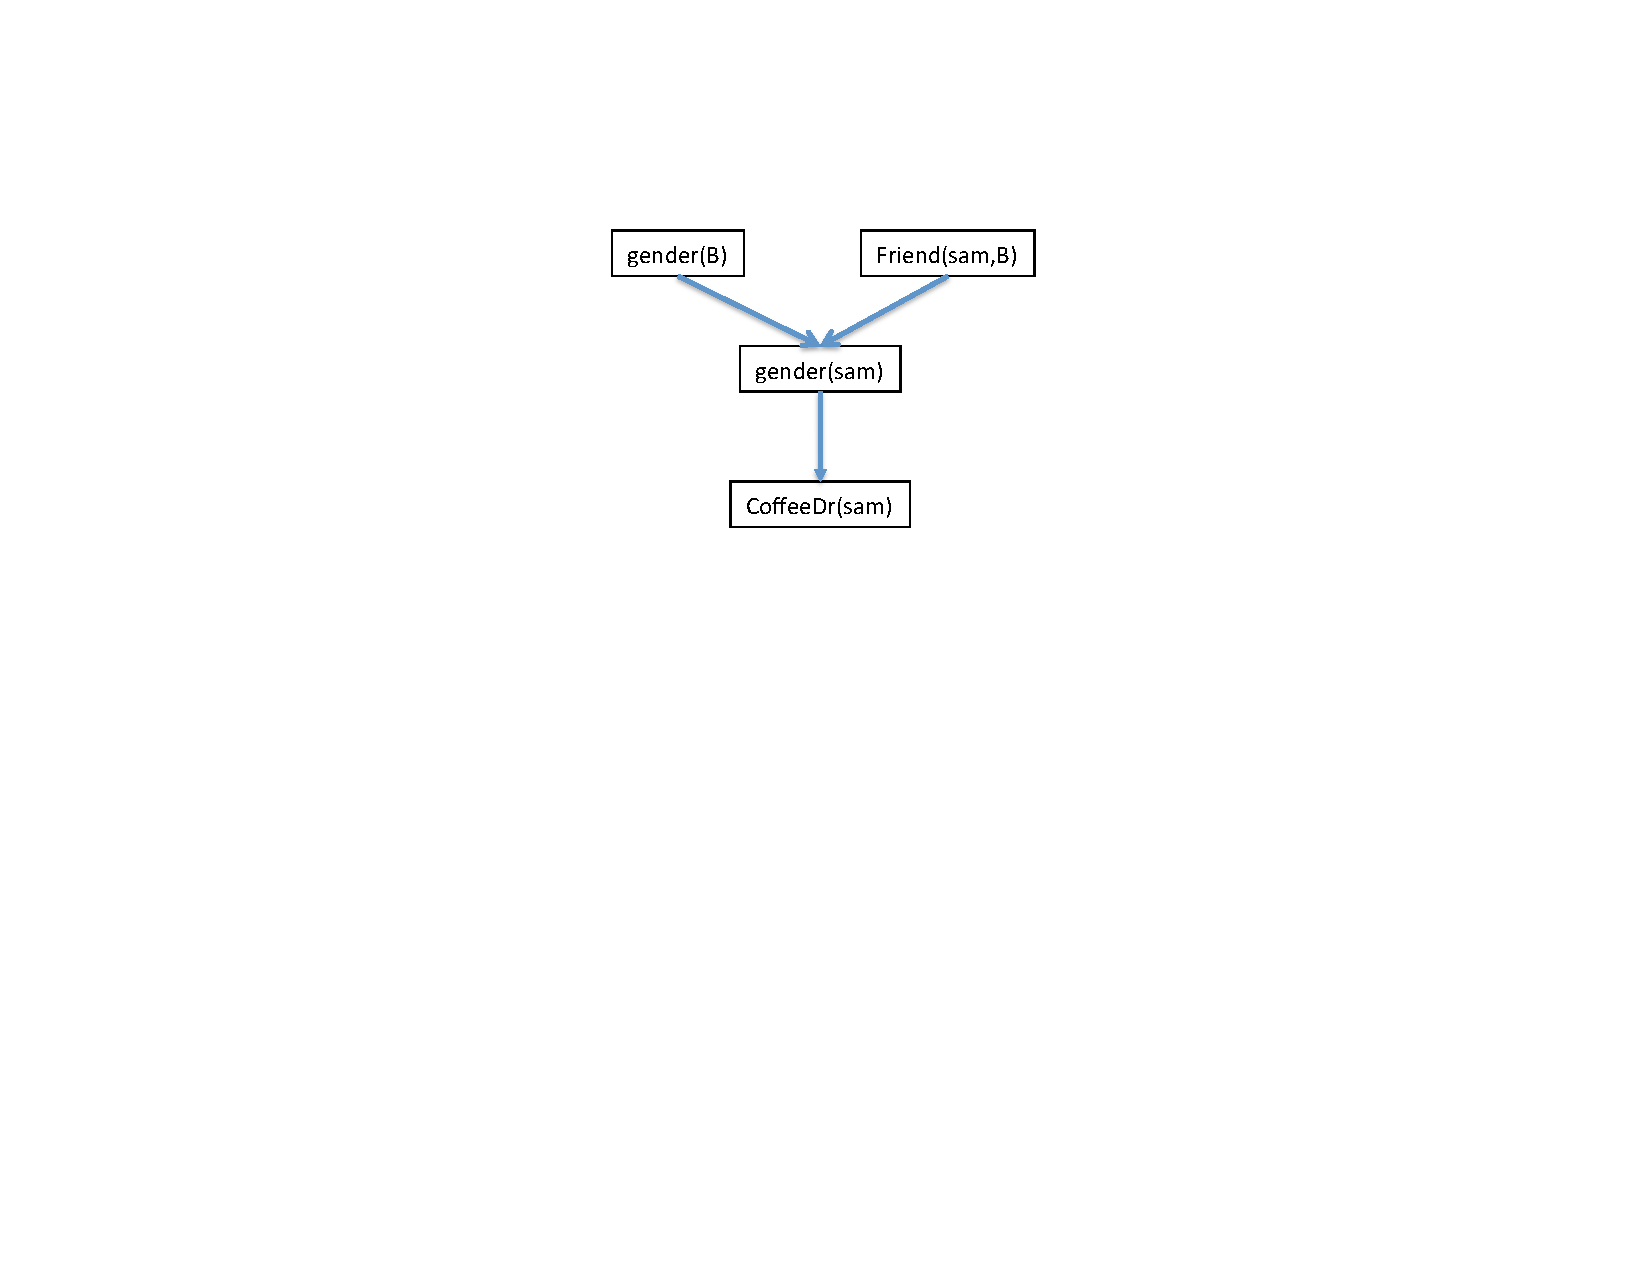
\includegraphics{figures/regression-graph}
%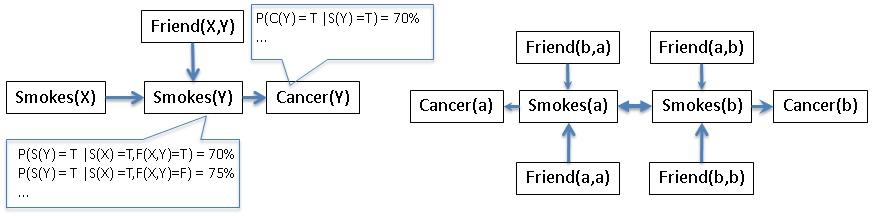
\includegraphics[width=2 \textwidth]{combine1.jpg}
}
\caption{Graphical representation of partial grounding for the target node $\it{gender}(sam)$. The graph results from instantiating the population variable $\A$ with the constant $sam$ in the template graph of Figure~\ref{fig:pbn}. Feature counts are computed with respect to the instantiated nodes. Notice that, for some nodes, this instantiation leads to only a {\em partial} grounding.
\label{fig:regress}}
\end{center}
\end{figure}

Normalizing feature counts to obtain feature frequencies must be done with care to take account of irrelevant features. Since irrelevant features receive log-difference weight 0, they are effectively pruned from the model, so their portion of the instantiation counts should be shifted to the relevant features, analogous to conditioning on relevant features. We therefore define the following two feature functions, where a feature is a family configuration.





\begin{description}
\item[Relevant Count]  The relevant count $\Relevant{\Cvar}$ is 0 if the family configuration is irrelevant; otherwise it is the instantiation count.
\item[Relevant Frequency] The relevant frequency of a feature is its relevant count, divided by the sum of all relevant counts for the same family.
\end{description}

%
%We define the relevant count $\Relevant{\Cvar}$ to be 0 if the query family configuration is irrelevant; otherwise it is the count. 

Algorithm~\ref{alg:relcount} describes the computation of relevant counts and relevant frequencies. Table~\ref{table:log-diff-example} gives examples. 
This completes our definition of the set of features, weights, and feature functions. All told, the resulting log-linear equation is as follows.





\begin{definition}[The Log-Difference Frequency Equation]\label{def:log-diff-freq-eq}
\begin{eqnarray*}
  \Gprob{\FG{\Ground{\TI}} = \TV} {\QC} &\propto & \exp(\ln \jprob{\TT = \TV} + \\
 \sum_{\UT} \sum_{\UV,\Prange{\UT}}   
\qquad \left[ \ln \cprob{\UT = \UV}{\Pa{\UT} = \Prange{\UT}} - \ln \jprob{\UT = \UV} \right] &
    \cdot &
    \Relfreq{\Appendterm{\Ground{\UI}  = \UV} {\Ground{\Pa{\UI}} = \Prange{\UT}}} {\Qconj})
%\label{eq:log-diff-freq}
\end{eqnarray*}
where 
\begin{eqnarray*}
\UT &\mbox{varies over} &  \Setaddterm{\TT} {\Ch{\TT}}, \\
\UV & \mbox{varies over} & \Range{\UT}, \quad\mbox{and}\\
\Prange{\UT} & \mbox{varies over} &  \Range{\Pa{\UT}}.
\end{eqnarray*}
\end{definition}


\begin{algorithm}[htbp]
%\linesnumbered
\SetKwData{Calls}{Calls}
\SetKwData{Notation}{Notation}
%\begin{algorithmic}
%{\footnotesize
%\STATE {\em Input}: Database $\D$ with $\etable_1,..\etable_e$ entity tables, functors $\F$, variable number bound $\varbound$.
\KwIn{Template Bayes Net $\BN$; Query $\Gprob{\FG{\Ground{\TI}} = \TV} {\QC} = ?$; Feature $F = \Appendterm{\UI  = \UV} {\Pa{\UI} = \Prange{\UT}$}}
%Feature $F = \Appendterm{\Ground{\UI}  = \UV} {\Ground{\Pa{\UI}} = \Prange{\UT}}$}
\KwOut{Relevant Feature Count $\Relcount{\Appendterm{\Ground{\UI}  = \UV} {\Ground{\Pa{\UI}} = \Prange{\UT}}} {\QC,\Ground{\TI} = \TV}$}
\begin{algorithmic}[1]
	\IF{the feature $F$ is not relevant in $\BN$}
	\STATE \Return 0.
	\ELSE
	\STATE Partially Ground Conjunction $C := (\Appendterm{\Ground{\UI}  = \UV} {\Ground{\Pa{\UI}} = \Prange{\UT}})$.
	\STATE Complete Conjunction $\DB := (\QC,\FG{\Ground{\TI}} = \TV)$.
	\STATE \Return $\Relcount{C}{\DB} :=$ $\Count{C}{\DB}$.
		\ENDIF \\
	%\STATE	
	\KwOut{Relevant Feature Frequency}
	\STATE $\it{Total\_Relevant\_Count}$ := $\sum_{\UV',\Prange{\UT}'}\Relcount{\Appendterm{\Ground{\UI}  = \UV'} {\Ground{\Pa{\UI}} = \Prange{\UT}'}} {\Qconj}$
	\STATE \Return $\Relfreq{C}{\DB}:=$ $\Relcount{C}{\DB}/\it{Total\_Relevant\_Count}$.
\end{algorithmic}
%\label{alg:cpt}
\caption{Computing Feature Functions: Relevant Counts and Relevant Frequencies. Feature = Query Family Configuration. \label{alg:relcount}}
\end{algorithm}



\begin{table}

%\resizebox{1.1\textwidth}{!}{
\begin{tabular}{lrlrrrr|rr}
%%%%%% DO NOT MODIFY THIS FILE DIRECTLY %%%%%%
%%%%%% IT IS GENERATED BY apply-eqs.py %%%%%%
\\\hline
{\setlength{\tabcolsep}{0pt}\begin{tabular}{l}Child \\Value \end{tabular}}&{\setlength{\tabcolsep}{0pt}\begin{tabular}{l} Prior \\ Prob. \end{tabular}}&Parent State&{\setlength{\tabcolsep}{0pt}\begin{tabular}{l} Cond. \\ Prob.\end{tabular}}&$w\;\;$&$\Relevant{\Fvar}$&$w \times \Relevant{\Fvar}$&$\Relevant{\Cvar}$&$w \times \Relevant{\Cvar}$ \\\hline
$cd(sam) = \true$&$0.70\;$&{\setlength{\tabcolsep}{0pt}\begin{tabular}{l}$ g(sam) = \Woman$\end{tabular}}&$0.80\;\,$&$0.13$&$1.0$&$0.13\;\;$&$1$&$0.13\;\;$ \\
$cd(sam) = \false$&$0.30\;$&{\setlength{\tabcolsep}{0pt}\begin{tabular}{l}$g(sam) = \Woman$ \end{tabular}}&$0.20\;\,$&$-0.40$&$0.0$&$0.00\;\;$&$0$&$0.00\;\;$ \\
$g(sam) = \Woman$&$0.45\;$&{\setlength{\tabcolsep}{0pt}\begin{tabular}{l}$ g(B) = \Woman,$\\ $F(sam,B) = \true$\end{tabular}}&$0.55\;\,$&$0.20$&$0.4$&$0.08\;\;$&$40$&$8.02\;\;$ \\
$g(sam) = \Woman$&$0.45\;$&{\setlength{\tabcolsep}{0pt}\begin{tabular}{l}$ g(B) = \Man,$\\ $ F(sam,B) = \true$\end{tabular}}&$0.37\;\,$&$-0.19$&$0.6$&$-0.11\;\;$&$60$&$-11.74\;\;$ \\
$g(sam) = \Woman$&$0.45\;$&{\setlength{\tabcolsep}{0pt}\begin{tabular}{l} n/a\end{tabular}}&$\mathrm{n/a}\;\,$&$-0.79$&$1.0$&$-0.79\;\;$&$1$&$-0.79\;\;$ \\\hline
\multicolumn{6}{l}{Sum ($\ln \Gprob{\it{gender}(sam) = \Woman} {\QC}$)}&$-0.70\;\;$&&$-4.38\;\;$ \\\hline
$cd(sam) = \true$&$0.70\;$&{\setlength{\tabcolsep}{0pt}\begin{tabular}{l}$ g(sam) = \Man$\end{tabular}}&$0.60\;\,$&$-0.15$&$1.0$&$-0.15\;\;$&$1$&$-0.15\;\;$ \\
$cd(sam) = \false$&$0.30\;$&{\setlength{\tabcolsep}{0pt}\begin{tabular}{l}$ g(sam) = \Man$\end{tabular}}&$0.40\;\,$&$0.28$&$0.0$&$0.00\;\;$&$0$&$0.00\;\;$ \\
$g(sam) = \Man$&$0.55\;$&{\setlength{\tabcolsep}{0pt}\begin{tabular}{l}$ g(B) = \Woman,$\\ $F(sam,B) = \true$\end{tabular}}&$0.45\;\,$&$-0.20$&$0.4$&$-0.08\;\;$&$40$&$-8.02\;\;$ \\
$g(sam) = \Man$&$0.55\;$&{\setlength{\tabcolsep}{0pt}\begin{tabular}{l}$ g(B) = \Man,$\\ $ F(sam,B) = \true$\end{tabular}}&$0.63\;\,$&$0.13$&$0.6$&$0.08\;\;$&$60$&$8.14\;\;$ \\
$g(sam) = \Man$&$0.55\;$&{\setlength{\tabcolsep}{0pt}\begin{tabular}{l} n/a \end{tabular}}&$\mathrm{n/a}\;\,$&$-0.59$&$1.0$&$-0.59\;\;$&$1$&$-0.59\;\;$ \\\hline
\multicolumn{6}{l}{Sum ($\ln \Gprob{\it{gender}(sam) = \Man} {\QC}$)}&$-0.75\;\;$&&$-0.63\;\;$ \\\hline

\end{tabular}
%}
\caption{Applying the log-difference frequency equation with the BN of Figure~\ref{fig:pbn} to compute $\Gprob{\it{gender}(sam) = \Woman} {\QC}$ and $\Gprob{\it{gender}(sam) = \Man} {\QC}$. Each row represents a feature/family configuration. For the sake of the example we suppose that the conjunction $\QC$ specifies that Sam is a coffee drinker, has 60 male friends, and 40 female friends.
The last two columns show the result of replacing frequencies by counts (the log-difference count equation in Section~\ref{sec:alternatives}).}
\label{table:log-diff-example}
\end{table}



\subsection{Discussion: Advantages of weights as log-differences of Bayes parameters}

Using Bayes nets in log-difference form is more scalable and interpretable than previous inference methods:

\point{(1)~Interpretable features/structure} General log-linear weights learned from data can be difficult to interpret, as they may reflect complex interactions between different correlated features. In contrast, a Bayes net parameter can be interpreted as a conditional probability, and reflects local statistics restricted to a family of nodes. 
%With maximum likelihood estimation, the conditional probabilities can be interpreted in terms of empirical frequencies observed in a relational structure.

\point{(2)~Interpretable weights/scale} The log-difference transformation of the Bayes parameters means that weights can be interpreted as usual in a log-linear model: a positive weight indicates positive relevance (the parent values raise the probability of a child value), a negative weight as negative relevance (parent values lower the child value probability), and a zero weight as irrelevance. 

\point{(3)~Scalable weight learning} The Bayes net parameters can be estimated using the empirical conditional frequencies observed in an input dataset $\FG{\D}$: The parameter estimate for a family configuration is the number of instantiations of that family configuration in $\FG{\D}$, divided by the sum of all instantiation counts for that family that agree on the parent values and vary the child values. In our notation, the estimate is defined by

\newcommand{\CTPa}{\Count{\Appendterm{\TT = \TV} {\Pa{\TT} = \Prange{\TT}}}  {\FG{\D}}}
\newcommand{\CTPb}{\Count{\Appendterm{\TT = \TV'} {\Pa{\TT} = \Prange{\TT}}}  {\FG{\D}}}

\begin{equation} \label{eq:frequencies}
\estcprob{\TT = \TV} {\Pa{\TT} = \Prange{\TT}} {\FG{\D}} = 
    \frac{\CTPa}
           {\sum_{\TV' \in \Range{\TT}}\CTPb}.
\end{equation}

A theoretical justification for using the observed conditional frequencies is that these estimates maximize a pseudo-likelihood function that measures how well a template BN matches an input dataset \cite{Schulte2011,Schulte2013}. The pseudo-likelihood can be interpreted as the expected value of the log-likelihood of a random grounding of the BN nodes in the template model.
%, and applying the standard BN product formula to compute a joint log-likelihood for this random instantiation.


\point{(4)~Compatibility with regularization} Because 0 is the neutral point on the scale, the log-difference formulation is compatible with standard methods to regularize weights towards zero~\cite{Huynh2008,Domingos2009}.  
%For example, the L1-norm $\ln \cprob{\UT = \UV}{\Pa{\UT} = \Prange{\UT}} - \ln \jprob{\UT = \UV}$ can be used to smooth parameter estimates. 

Frequency estimates can be viewed as a type of \defterm{lifted learning}, the approach of using only the sufficient statistics for a dataset rather than an iteration over ground facts. The computational cost of lifted learning scales well in both data size and the number of parameters in the model \cite{Schulte2013}. 

%The Gibbs conditional probabilities defined by the log-difference equation can be derived from different approaches to relational inference. 
In Section~\ref{sec:random} we prove that, given mild assumptions about the Bayes net structure, the log-difference value is equivalent to a random grounding definition: the expected value of choosing a random grounding of the BN nodes in the template model, and applying the BN log-linear equation~\eqref{eq:bn-mb} to this random grounding. Thus the log-difference model can be viewed as an application of the random selection semantics for template Bayes nets \cite{Schulte2013}.
%In Section~\ref{sec:other} we show that the log-difference equation is equivalent to the following method: 1) for all query family configuration with the same child node, compute their {\em geometric mean}. 2) Multiply together the geometric means.  In our view, the fact that alternative approaches lead to the same result mutually reinforces each.  
Before we describe the equivalence to random grounding inference, we provide experiments to evaluate our model's predictive performance.
The next section presents several bases for comparison, alternative log-linear regression equations that can be computed in closed-form from a Bayes net template. 



\section{Alternative Log-Linear Equations}\label{sec:alternatives}
We consider three alternatives to the log-difference frequency equation. First, an alternative method for computing weights from Bayes net parameters: replace the log-difference of conditional probabilities with log-conditional probabilities. This is exactly the weight computation used in the BN log-linear equation~\eqref{eq:bn-mb}. 
Second, a different feature function: Replace relevant feature frequencies by relevant counts. These alternatives define 4 different equations, shown in Table~\ref{table:weights-predictors-equations}. Table~\ref{table:equation-examples} shows the prediction of the gender of $sam$ for each equation.
% with the detailed computations in Appendix~\ref{app:proofs}.


%Our experiments compare the log-difference equation~\eqref{eq:log-diff} with a number of alternative equations. Table~\ref{table:equations} lists their definitions. 

\begin{table}[htdp]
%\vspace{-2cm}
\caption{Log-Linear Regression Equations for Relational Data.}
\begin{center}
\begin{tabular}{|l|l|c|c|}
\hline
%Name & Definition : $\Gprob{\FG{\Ground{\TI}} = \TV} {\DB} = $ \\ \hline \hline
Name & Weight & Function & \begin{tabular}{c} Offset \\ $w_0$ \end{tabular} \\\hline
Log-difference frequency & $\ln \cprob{\UT = \UV}{\Pa{\UT} = \Prange{\UT}} - \ln \jprob{\UT = \UV}$ & $\Relevant{\Fvar}$ & Yes \\
Log-cp frequency & $ \ln \cprob{\UT = \UV}{\Pa{\UT} = \Prange{\UT}} $ & $\Relevant{\Fvar} $ & No \\
Log-difference count & $ \ln \cprob{\UT = \UV}{\Pa{\UT} = \Prange{\UT}} - \ln \jprob{\UT = \UV} $ & $\Relevant{\Cvar} $ & Yes \\
Log-cp count & $ \ln \cprob{\UT = \UV}{\Pa{\UT} = \Prange{\UT}} $ & $\Relevant{\Cvar}$ & No \\ \hline

\end{tabular}
\end{center}
\label{table:weights-predictors-equations}
\end{table}%

\begin{table}[htdp]
\vspace{-1cm}
\caption{The log-probability difference for the gender of $sam$ in our running example, according to each of the equations. Notice that the two frequency equations give the same log-ratio, as entailed by Theorem~\ref{prop:log-diff}. The frequency equations give the intuitively correct answer, that Sam is most likely to be a woman. The two count equations give the opposite answer, with log-cp weights by a greater margin than log-difference weights.}
\begin{center}
\begin{tabular}{|l|r|r|r|}
\hline
Name & \multicolumn{2}{c|}{log-linear sum for} & log-ratio= \\
 & $\Gprob{sam = \Woman} {\DB} $ & $\Gprob{sam = \Man} {\DB} $ & column1 - column2
% \begin{tabular}{l}
% log-ratio = \\ 
% column1 - column2 \end{tabular} 
 \\ \hline
Log-difference frequency & -0.70 & -0.75 & 0.05 \\
Log-cp frequency & -1.06 & -1.10 & 0.05 \\
Log-difference count & -4.38 & -0.63 & -3.75 \\
Log-cp count & -83.79 & -60.17 & -23.62 \\
\hline
\end{tabular}
\end{center}
\label{table:equation-examples}
\end{table}%


\subsection{The Frequency Equations} The frequency equation in the second row of Table~\ref{table:weights-predictors-equations} uses the log-conditional probabilities of a child value given a parent configuation as weights. It does not normalize the conditional probabilities by the marginal probability of the child value, nor does it include an offset. 
%This weight choice agrees with the standard way of converting a BN to a log-linear model for nonrelational data, the so-called moralization  method \cite[12.5.3]{Domingos2007}, \cite{Lauritzen1996}. This is the method for converting a Bayes net conversion to a log-linear model recommended by the Alchemy system %\cite{bib:bayes-convert}. 
%\footnote{Moralization connects all spouses that share a common child, and makes all edges in the resulting graph undirected. Each family in the Bayes net becomes a clique in the moralized structure. For each state of each family clique, define the clique potential in the Markov net to be the conditional probability of the child given its parents.} 
Despite these differences, the two regression equations make the same prediction. This is true in general:

\begin{theorem} \label{prop:log-diff} Frequency regression with log-conditional probabilities is equivalent to frequency regression with log-differences.
\end{theorem}

\begin{proof} See the Appendix. %~\ref{app:proofs}.
\end{proof}


Although the two frequency equations are mathematically equivalent, the log-difference weights are more interpretable than the log-conditional probability weights: With log-cps, all weights are negative or zero, with a zero weight indicating infinite importance, rather than irrelevance.


\subsection{The Count Equations} \label{sec:countequations}


The count equations replace relevant frequencies with relevant counts as feature functions, but are otherwise the same as their frequency counterparts. While normalizing counts to frequencies is the most direct and effective way to address the imbalance problem, to some extent the scales of different feature counts can be balanced through the weights, by assigning weights of smaller magnitude to features that tend to have larger counts. The example of Table~\ref{table:equation-examples} suggests that log-difference weights scale counts more effectively than log-cp weights. In the next section we report empirical results that confirm this finding on real-world benchmark datasets. We also report results for when weights are learned using general log-linear optimization methods, rather than computed from Bayes net parameters. These optimized weights also exhibit scaling effects, where features with larger counts tend to be assigned weights of smaller magnitude.


%

\section{Empirical Comparison of Bayes Net Log-linear Equations}\label{sec:empirical-comparison}

Our first set of experiments compared the predictive accuracy of different Bayes net regression equations. The next section describes experiments comparing the Bayes net methods with general weight learning for log-linear models. 

\subsection{Experimental Conditions and Metrics}\label{sec:conditions}

All experiments were done on with 8GB of RAM and a single Intel Core 2 QUAD Processor Q6700 with a clock speed of 2.66GHz (there is no hyper-threading on this chip). The operating system was Linux Centos 2.6.32. Code was written in Java, JRE 1.7.0. All code and datasets are available~\cite{bib:jbnsite}. 

\subsubsection{Datasets}

We describe the datasets in terms of their representation as databases with tables. The databases follow an Entity-Relationship (E-R) design \cite{Ullman1982}. An E-R schema can be translated into our function-based logical notation as follows: Entity sets correspond to populations, descriptive attributes to functions, relationship tables to predicates, and foreign key constraints to type constraints on the arguments of relationship predicates.
%
We used %one synthetic and 
5 benchmark real-world databases from prior work~\cite{Schulte2012}. 
%The databases are fairly complex, so the experiments are computationally demanding, especially the Alchemy inference component, which needs to be applied to all groundings of all descriptive attributes to compute average predictive performance. The databases and their main characteristics are as follows. 
% and on-line sources such as \cite{bib:jbnsite}.
%In this paper we report the average result over all subdatabases in this paper and leave the evaluation of how models should evolve based on the size of data to an extension of the work in a journal paper. 


%{\em University Database.} We manually created a small dataset, based on the schema given in Table~\ref{table:university-schema}.
%The dataset is small and is used as a toy example for testing purposes. There are three entity tables, Student, Course, Professor, and 2 relationship tables RA and Registered.
%The entity tables contain 38 students, 10 courses, and 6  Professors. The $\reg$ table has 92 rows and the $\it{RA}$ table has 25 rows. %This dataset is translated into 513 ground atoms.

\begin{description}

\item[MovieLens Database] This is a standard dataset from the UC Irvine machine learning repository. 
% \cite{Schulte2012}.
%The schema for the dataset is shown in Table \ref{}.
It contains two tables representing entity sets: User with 941 tuples and Item (Movies) with 1,682 tuples.
The User table has 2 descriptive attributes, $\age$ and $\it{gender}$. We discretized the attribute $\age$ into three equal-frequency bins. The table Item represents information about the movies. It has 17 Boolean attributes that indicate the genres of a given movie. There is one relationship table Rated corresponding to a Boolean predicate. The Rated contains Rating as descriptive attribute; 80,000 ratings are recorded.  We performed a preliminary data analysis and omitted genres that have only weak correlations with the rating or user attributes, leaving a total of three genres (Drama, Horror, Action).
%
%The full dataset contains 170,143 ground atoms and is too big for Alchemy to perform learning. We made small subsamples to make the experiments feasible. Subsampling 100 Users and 100 Items transforms to an Alchemy input file with 3,485 ground atoms. Structure learning with Alchemy takes around 30 min.
%Subsampling 300 Users and 300 Items transforms to an Alchemy input file with 27,134 ground atoms. Structure learning with Alchemy takes about 2 days to run.
%The full table with 100,000 ratings exceeded the memory limits of Tetrad, so we randomly picked 40\% of the ratings of the relationship table as input data.

\item[Mutagenesis Database] This dataset is widely used in Inductive Logic Programming research \cite{Srinivasan1996}. %It contains 4 tables total to 15218 tuples. 
We used a previous discretization \cite{Schulte2012}.
Mutagenesis has two entity tables, Atom with 3 descriptive attributes, and Mole (decribing molecules), with 5 descriptive attributes. 
%including two attributes that are discretized into ten values each (logp and lumo).
There are two relationship tables, MoleAtom, indicating which atoms are parts of which molecules, and Bond, which relates two atoms and has 1 descriptive attribute. 
%The full dataset, with 35,973 ground atoms, crashed Alchemy with both structure  and parameter learning. A subsample with 5,017 ground atoms did not terminate for structure learning, but weight learning was feasible. The computational difficulties of Alchemy compared to the MovieLens dataset are  due to the high number of descriptive attributes.
%%another subsample with
%Representing a relationship between entities from the same table in a parametrized Bayes net requires using two or more variables associated with the same population (e.g., $\it{Bond}(\A_{1},\A_{2}))$.
%(Techreport 2009) describes a straightforward extension of Algorithm~\ref{alg:structure} for this case, which we applied to the Mutagenesis dataset.\footnote{Reference omitted for blind review.}
%We also tested our method on the Financial dataset with similar results, but omit a discussion due to space constraints.

\item[Hepatitis Database] This data is a modified version of the PKDD02 Discovery Challenge database \cite{Frank2007}. %, which includes removing tests with null values. 
The database contains information on laboratory examinations of 771 hepatitis B- and C-infected patients, taken
between 1982 and 2001. The data are organized in 7 tables (4 entity tables,  3 relationship tables) with 16 descriptive attributes. They contain basic information about the patients, results of biopsy, information on interferon therapy, results of out-hospital examinations, and results of in-hospital examinations. 

\item[Mondial Database] 
%
%\textbf{Hassan: which version did you use? The full one from http://www.dbis.informatik.uni-goettingen.de/Mondial/mondial-ER.pdf or Bahareh's?} 
%
This dataset contains data from multiple geographical web data sources. 
%Our dataset contains 4 entity tables, $\it{Country},\it{Continent},\it{Economy},\it{Government}$, where the latter three are related to Country by many-one relationships, and one relationship table $\it{Borders}$ that relates two countries.
%This dataset contains data from multiple geographical Web data sources \cite{mondial}. 
We follow the modification of She~\etal~\cite{wangMondial}, and use a subset of the tables and disretized features: 2 entity tables, $\it{Country},\it{Economy}$. The descriptive attributes of Country are continent, government, percentage, majority religion, population size. The descriptive attributes of Economy are inflation, gdp, service, agriculture, industry. A relationship table Economy\_Country specifies which country has what type of economy. A self-relationship table Borders relates two countries.
  %$\it{Country},\it{Continent},\it{Economy},\it{Government}$, where the latter three are related to Country by many-one relationships, and one relationship table $\it{Borders}$ that relates two countries. Our dataset includes a self-relationship table Borders that relates two countries.



\item[UW-CSE database] This dataset lists facts about the Department of Computer Science and Engineering at the University of Washington, such as entities (e.g., $Student$, $Professor$) and their relationships (i.e. $AdvisedBy$, $Publication$).
% \cite{Domingos2007}. 
%The total number of ground atoms is 4,106,841. The database contained a total of 3380 ground atoms. 

\end{description}

\subsubsection{Prediction Metrics}
We evaluate the algorithms using classification
accuracy and conditional log likelihood (CLL). These metrics have been used in previous evaluations of MLN learning~\cite{Domingos2007,Schulte2012}.  For each fact $\FG{\TI} = \TV$ in the test dataset, we evaluate the accuracy of the predicted Gibbs probability $\Gprob{\FG{\TI} = \TV} {\QCtarget}$, where $\QCtarget$ is a complete conjunction for all ground terms other than $\FG{\TI}$. Thus $\QCtarget$ represents the values of the input variables as specified by the test dataset.
For classification accuracy, a model's prediction is scored as correct if the true value of the ground term in the test dataset receives the highest Gibbs probability. 
CLL is the average of the logarithm of the Gibbs probability for each fact in the test dataset. Thus $\exp(CLL)$ is the geometric mean of the Gibbs probabilities.\footnote{The geometric mean of a list of numbers $x_{1},\ldots,x_{n}$ is $(\prod_{i} x_{i})^{1/n}$.}
Both metrics are reported as averages over all functors that represent descriptive attributes. We do not use Area Under Curve, as it mainly applies to binary values, and most of the attributes in our datasets are nonbinary.
The learning methods were evaluated using 5-fold cross-validation. Each database was split into 5 folds by randomly selecting entities from each entity table, and restricting the relationship tuples in each fold to those involving only the selected entities  (i.e., subgraph sampling~\cite{Frank1977,Schulte2012}). The models were trained on 4 of the 5 folds, then tested on the remaining one. All results are averages from 5-fold cross validation, over all descriptive attributes in the database. 


\subsection{Learning the Bayes Net Structure and Parameters}

All the methods compared in this experiment require a prior Bayes net structure and parameters.
To obtain the structure, the learn-and-join algorithm~\cite{Schulte2012} was applied to each benchmark database. The parameters were computed from the empirical conditional frequencies in the database (Eq.~\ref{eq:frequencies}) using previously-published algorithms~\cite{Schulte2013}. The resulting structure and parameters were used for all methods in this experiment. Table~\ref{table:methods} shows the 3 log-linear equations compared with abbreviations. To determine the set of relevant features, we eliminated conjunctions that involved negated relationships (e.g., $\it{Friend}(\A,\B) = \false$), for the following reasons. (i) We inspected the log-difference weights for these features and found them close to 0. Eliminating such weights approximates regularization. We leave a full regularization approach for eliminating irrelevant features for future work. (ii) Eliminating information from unrelated entities is standard practice in statistical-relational learning \cite{Natarajan2008,Heckerman+al:SRL07}. (iii) Log-linear weight learning methods (e.g., Alchemy, see Section~\ref{sec:general-weights}) do not scale to our datasets when features with negated relationships are included (because of the difficulty of computing sufficient statistics for such features). 

 

\begin{table}[htdp]
\caption{The Bayes net log-linear equations compared in our experiments; cf. Table~\ref{table:weights-predictors-equations}. Theorem~\ref{prop:log-diff} shows that the log(cp) + frequency  and log-diff + frequency  are equivalent.}
\begin{center}
%^\resizebox{0.5\textwidth}{!}{
\begin{tabular}{l l|c|c|}
\cline{3-4}
& & \multicolumn{2}{| c |}{Feature Function} \\\cline{3-4}
& & Count & Frequency \\\hline
\multicolumn{1}{|l|}{\multirow{2}{*}{Weights}}  & 
\multicolumn{1}{|l|}{Log-CPs} & log(cp) $+$ count & \multirow{2}{*} {log-diff $+$ freq} \\
\multicolumn{1}{|l}{} &
\multicolumn{1}{|l|}{Log-diff.} & log-diff $+$ count & \\\hline
\end{tabular}
%}
\end{center}
\label{table:methods}
\end{table}%




\subsection{Results} 

Table~\ref{table:bn} summarizes the results for the Bayes net regression equations. 
The numbers represent an average over many individual scores, one for each fact
%ground literal 
in the database. 
For instance in the biggest dataset, MovieLens, the average is over a total of 170,000 scores; see Table~\ref{table:learn-times}. 

To aid interpretability, we also report the following transformation of CLL: prob. ratio = $\exp(CLL(method) - \exp(CLL(log(cp) + count))$,  where $\it{method}$ is one of log-diff $+$ count and log-diff $+$ frequency. This quantity represents the geometric mean, over all test facts, of the fact likelihood ratio of $\it{method}$  over the $log(cp) + count$ equation.
%the likelihood assigned by the $log(cp) + count$ equation. 
For instance, the value of 1.05 for the dataset UW and the log-diff $+$ count method means that on (geometric) average, the likelihood that the log-diff $+$ count method assigns to the correct value for the target node is 1.05 times that assigned by the log-(cp) $+$ count method.


 
\begin{table}[thbp]
\caption{Conditional log-likelihood (log-probabilities) and classification accuracy (in percent) of Bayes net regression predictions. We show averages and standard deviations. The probability ratios can be interpreted as the geometric average ratio of likelihoods assigned by the model to the true target node value.}

%\resizebox{0.5\textwidth}{!}{

\begin{center}
%\resizebox{0.5\textwidth}{!}{
\begin{tabular}{|l|c|c|c|c|c|}
\hline
Accuracy& UW & Mondial & MovieLens & Mutagenesis & Hepatitis \\\hline
log(cp) $+$ count & 78 $\pm$ 0.08 & 40 $\pm$ 0.05 & 64 $\pm$ 0.01 & 62 $\pm$ 0.05 & 49 $\pm$ 0.03 \\
log-diff $+$ count & \textbf{81} $\pm$ 0.06 & \textbf{45} $\pm$ 0.04 & 62 $\pm$ 0.02 & \textbf{67} $\pm$ 0.03 & \textbf{55} $\pm$ 0.02 \\
log-diff $+$ freq & \textbf{81} $\pm$ 0.06 & \textbf{45} $\pm$ 0.04 & \textbf{65} $\pm$ 0.01 & \textbf{67} $\pm$ 0.03 & \textbf{55} $\pm$ 0.02 \\
\hline
\end{tabular}
\end{center}

\begin{center}
\begin{tabular}{|l|c|c|c|c|c|}
\hline
CLL & UW & Mondial & MovieLens & Mutagenesis & Hepatitis \\\hline
log(cp) $+$ count & -0.47 $\pm$ 0.10 & -1.47 $\pm$ 0.17 & -1.19 $\pm$ 0.07 & -0.84 $\pm$ 0.03 & -1.33 $\pm$ 0.07 \\
log-diff $+$ count & -0.42 $\pm$ 0.05 & -1.36 $\pm$ 0.11 & -1.10 $\pm$ 0.16 & -0.77 $\pm$ 0.03 & -1.20 $\pm$ 0.07\\
Prob. ratio & 1.05 & 1.12 & 1.09 & 1.07 & 1.14\\\hline
log-diff $+$ freq & \textbf{-0.41} $\pm$ 0.04 & \textbf{-1.34} $\pm$ 0.09 & \textbf{-0.71} $\pm$ 0.01 & \textbf{-0.73} $\pm$ 0.04 & \textbf{-1.07} $\pm$ 0.10\\
Ratio to ld-count & 1.01 & 1.02 & 1.48 & 1.04 & 1.14\\
\hline
\end{tabular}
%}
\end{center}
\label{table:bn}
\end{table}%


\subsection{Discussion} Frequency feature functions achieve top performance for  classification accuracy. However, classification scores are similar across the three methods, and the difference between frequencies and counts + log-difference weights is small ($<1\%$), except for a bigger improvement (3\%) on MovieLens. Whereas classification accuracy is a 0-1 loss function, CLL is continuous, so the frequency approach's balancing of factors has substantially more impact on CLL. With respect to CLL, we observe the following ranking of methods on each dataset: 
\begin{quote}
Frequency $>$ log-difference count $>$ count.
\end{quote} Therefore: \keypoint{Using Bayes net parameters, frequency feature functions outperform count feature functions, with both the log-cp and the log-diff weight computation methods.} This finding supports our hypothesis that using frequencies as feature functions is an effective way of addressing the imbalance problem.

\keypoint{Applied to feature counts, log-difference weights improve on log-conditional probabilities.} Our explanation for this finding is that log-difference weights are a heuristic for solving the imbalance problem, for the following reasons. 
Generally speaking, the number of instantiation count increases for a feature when the feature is based on longer relationship chains. In other words, (i) the number of instantiation counts increases with distance to the target entity.
 For instance, in the Bayes net of Figure~\ref{fig:pbn}, with target node $\it{gender}(sam)$, the feature $\it{CoffeeDrinker}(sam)$ is at distance 0 from Sam, and has instantiation count at most 1. The feature $\it{Friend}(sam,\B) = \true,\it{gender}(\B) = \Woman$ is at distance 1 from Sam (one link away), and its maximum instantiation count is the number of Sam's friends. A feature like $\it{Friend}(sam,\B) = \true, \it{Friend}(\B,\C) = \true, \it{gender}(\C) = \Woman$---referring to women friends of Sam's friends---is at distance 2 from Sam (two links away), and its maximum instantiation count is the number of friends of friends of Sam. We also expect that the correlation between Sam's gender and that of a friend will generally be stronger than than between Sam's gender and the gender of a friend of a friend. Therefore we can expect that (ii) the probabilistic association of the target node with related entities decreases with distance to the target entity. (iii) As the probabilistic association decreases, so does the log-difference weight since it measures the strength of the probabilistic association. Combining the observations (i), (ii), (iii) entails that features with high instantiation counts tend to have low log-difference weights. Therefore log-difference weights address the imbalance problem by tending to assign lower weight magnitudes to features with high instantiation counts. Table~\ref{table:heuristic} summarizes the quantities related to this analysis and how they relate to each other. 

\begin{table}[htdp]
\caption{Connections between different quantities for features that are consistent with the observed performance of count feature functions. 
%For typical datasets we expect that the feature instantiation count tends to increase with the relational distance of a feature to the target entity, while the correlation between target node value and the feature tends to decrease, and with it the log-difference weight.
}
\begin{center}
\begin{tabular}{|p{3cm}|p{3cm}p{3cm}p{3cm}|}
Distance to Target Entity & Feature Instantiation Count & Correlation with Target Attribute & Log-Difference Weight \\\hline
+ increases & + increases & - decreases & - decreases
\end{tabular}
\end{center}
\label{table:heuristic}
\end{table}%




\section{General Weight Learning Experiments}
\label{sec:general-weights}

The experiments in Section~\ref{sec:empirical-comparison} held the Bayes net structure and parameters constant and compared transformations of the BN parameters into log-linear weights. In this section we examine a setting where the same features are computed from the BN structure, but weights are {\em not} computed from the BN parameters. Instead weight values are optimized by a local search method. This experiment used the same conditions and metrics described in Section~\ref{sec:conditions}.  In addition to comparing predictive performance, we also report learning times.

To learn the weights, we applied the default training procedure of the Alchemy package \cite{Kok2009a}.  This procedure takes as input a set of features specified as logical formulas, and returns a weight for each formula. We followed the method recommended by the Alchemy group \cite{bib:bayes-convert} for converting a Bayes net structure to a Markov Logic Network structure: For each family configuration $\family_{ijk}$ in the BN, add a conjunction of literals that specifies the state. We also added unit clauses for each node-value combination, as recommended by the Alchemy group; unit clause weights can represent the bias weight of a log-linear equation.


%The Markov Logic Network (MLN) structure for weight learning was computed by the moralization procedure \cite[12.5.3]{Domingos2007}: convert a parametrized Bayes net to an MLN structure that contains,  for each family state $\family_{ijk}$ in the net, a conjunction of literals that specifies the state. This is the recommended procedure%~\cite{bib:bayes-convert} for converting a Bayes net to a Markov Logic Network.\footnote{We also added unit clauses for each node-value combination, as recommended by the Alchemy group.}  
%; see also Section~\ref{sec:other}. Weights learned by Alchemy are therefore appropriate for count regression. 
We refer to moralization+weight learning as the \defterm{MBN} method, for ``Moralized Bayes Net''   \cite{Khosravi2010}. 
MBN has been the state-of-the-art method for log-linear prediction with Bayes nets \cite{Schulte2012}. Figure~\ref{fig:mbn-flow} shows the program flow for the MBN method.
Markov Logic Network weight learning optimizes for log-linear inference with counts as feature functions~\cite{Schulte2011}. The prediction probabilities were computed exactly using the log-linear equation~\ref{eq:log-linear} with counts as feature functions. We used an exact computation rather than approximate inference
(e.g., MC-SAT), to avoid confounding the effect of the log-linear equation with that of inference implementation. Experiments with MC-SAT produced similar results. We also computed the results with frequencies as feature functions, which for optimized weights were very similar, so we do not present them. 


\begin{figure}[htbp]
\begin{center}

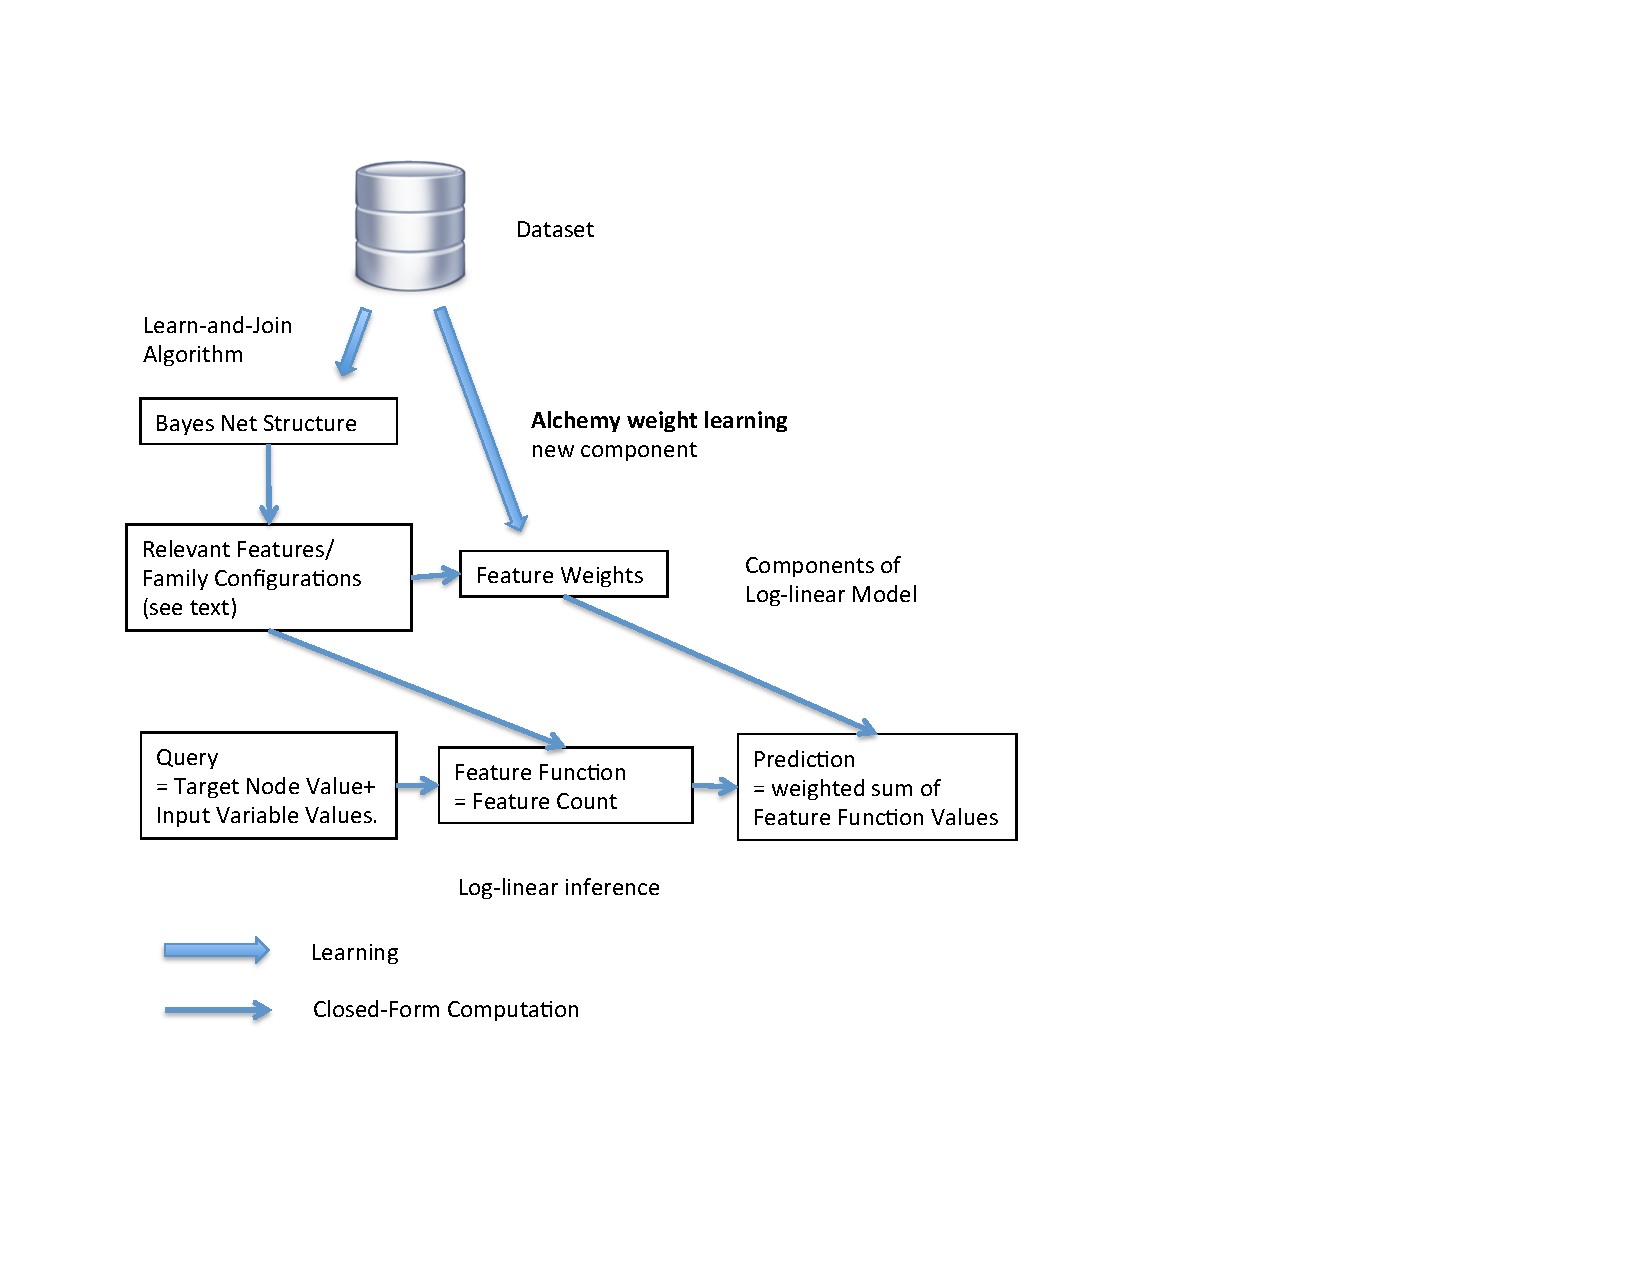
\includegraphics[width=0.7\textwidth]{figures/mbn-regress}
\caption{The MBN method: Program flow for computing relational Gibbs probabilities with general weight learning. A BN template structure is learned from the data using the learn-and-join algorithm. Relevant features are computed from the BN structure. Feature weights are computed by applying Markov Logic Network weight learning to the data. The Bayes net parameters are not estimated.}
\label{fig:mbn-flow}
\end{center}
\end{figure}



\subsection{Results}

\keypoint{The Bayes net frequency regression predictions are competitive with those from a model with optimized general weights.}

%%UW values are from Zhensong
\point{Accuracy} Table~\ref{table:mbn} shows the scores of the MBN method, together with the log-difference frequency results from Table~\ref{table:bn}. The log-difference frequency model scores slightly higher than the MBN weights on every dataset, with the biggest differences on Mutagenesis (5\%),  MovieLens (5\%) and Hepatitis (4\%). 

\begin{table}[thbp]

\caption{Conditional log-likelihood (log-probabilities) and classification accuracy (percent) of MBN and log-difference frequency predictions.}

\begin{center}

\begin{tabular}{|l|c|c|c|c|c|}
\hline
Accuracy& UW & Mondial & MovieLens & Mutagenesis & Hepatitis \\\hline
MBN & 80 $\pm$ 0.05 & 44 $\pm$ 0.04 & 60 $\pm$ 0.02 & 62 $\pm$ 0.02 & 51 $\pm$ 0.02 \\\hline
log-diff $+$ freq & \textbf{81} $\pm$ 0.06 & \textbf{45} $\pm$ 0.04 & \textbf{65} $\pm$ 0.03 & \textbf{67} $\pm$ 0.03 & \textbf{55} $\pm$ 0.02 \\
\hline
\end{tabular}
\end{center}


\begin{center}
\begin{tabular}{|l|c|c|c|c|c|}
\hline
CLL & UW & Mondial & MovieLens & Mutagenesis & Hepatitis \\\hline
MBN & -0.44 $\pm$ 0.07 & \textbf{-1.28} $\pm$ 0.07 & -0.79 $\pm$ 0.03 & -0.91 $\pm$ 0.09 & -1.18 $\pm$ 0.26 \\
log-diff $+$ freq & \textbf{-0.41} $\pm$ 0.04 & -1.34 $\pm$ 0.09 & \textbf{-0.71} $\pm$ 0.01 & \textbf{-0.73} $\pm$ 0.04 & \textbf{-1.07} $\pm$ 0.10 \\
Prob. ratio & 1.03 & 0.94 & 1.08 & 1.20 & 1.12\\
\hline
\end{tabular}
%}
\end{center}
\label{table:mbn}

\end{table}%


\point{CLL}
The log-difference frequency  model scores better than MBN model on UW, MovieLens, Mutagenesis and Hepatitis (probabilities 3--20\% higher) and scores slightly worse on Mondial (6\% lower probability); see Figure~\ref{fig:summarize}.

\begin{figure}[htbp]

\begin{center}
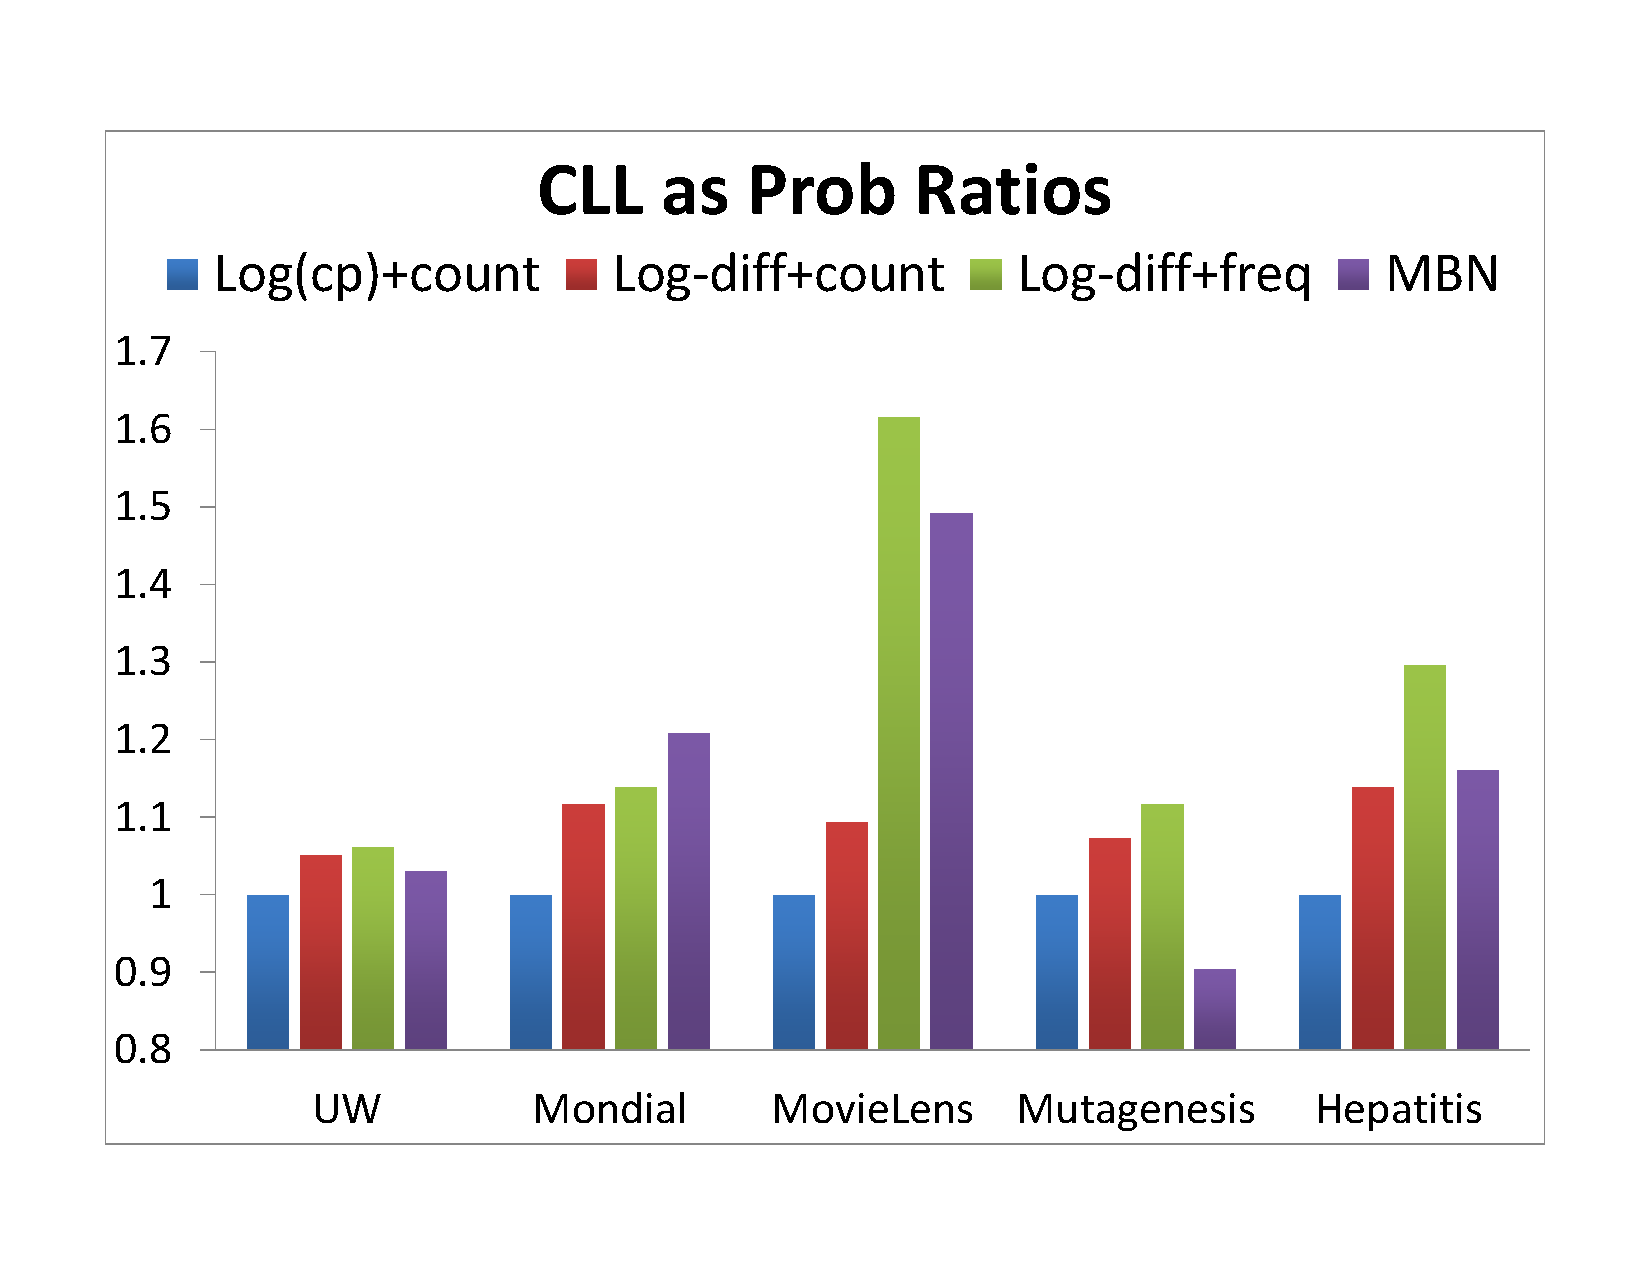
\includegraphics[width=0.6\textwidth]{CLL_Prob_Ratios_New}
%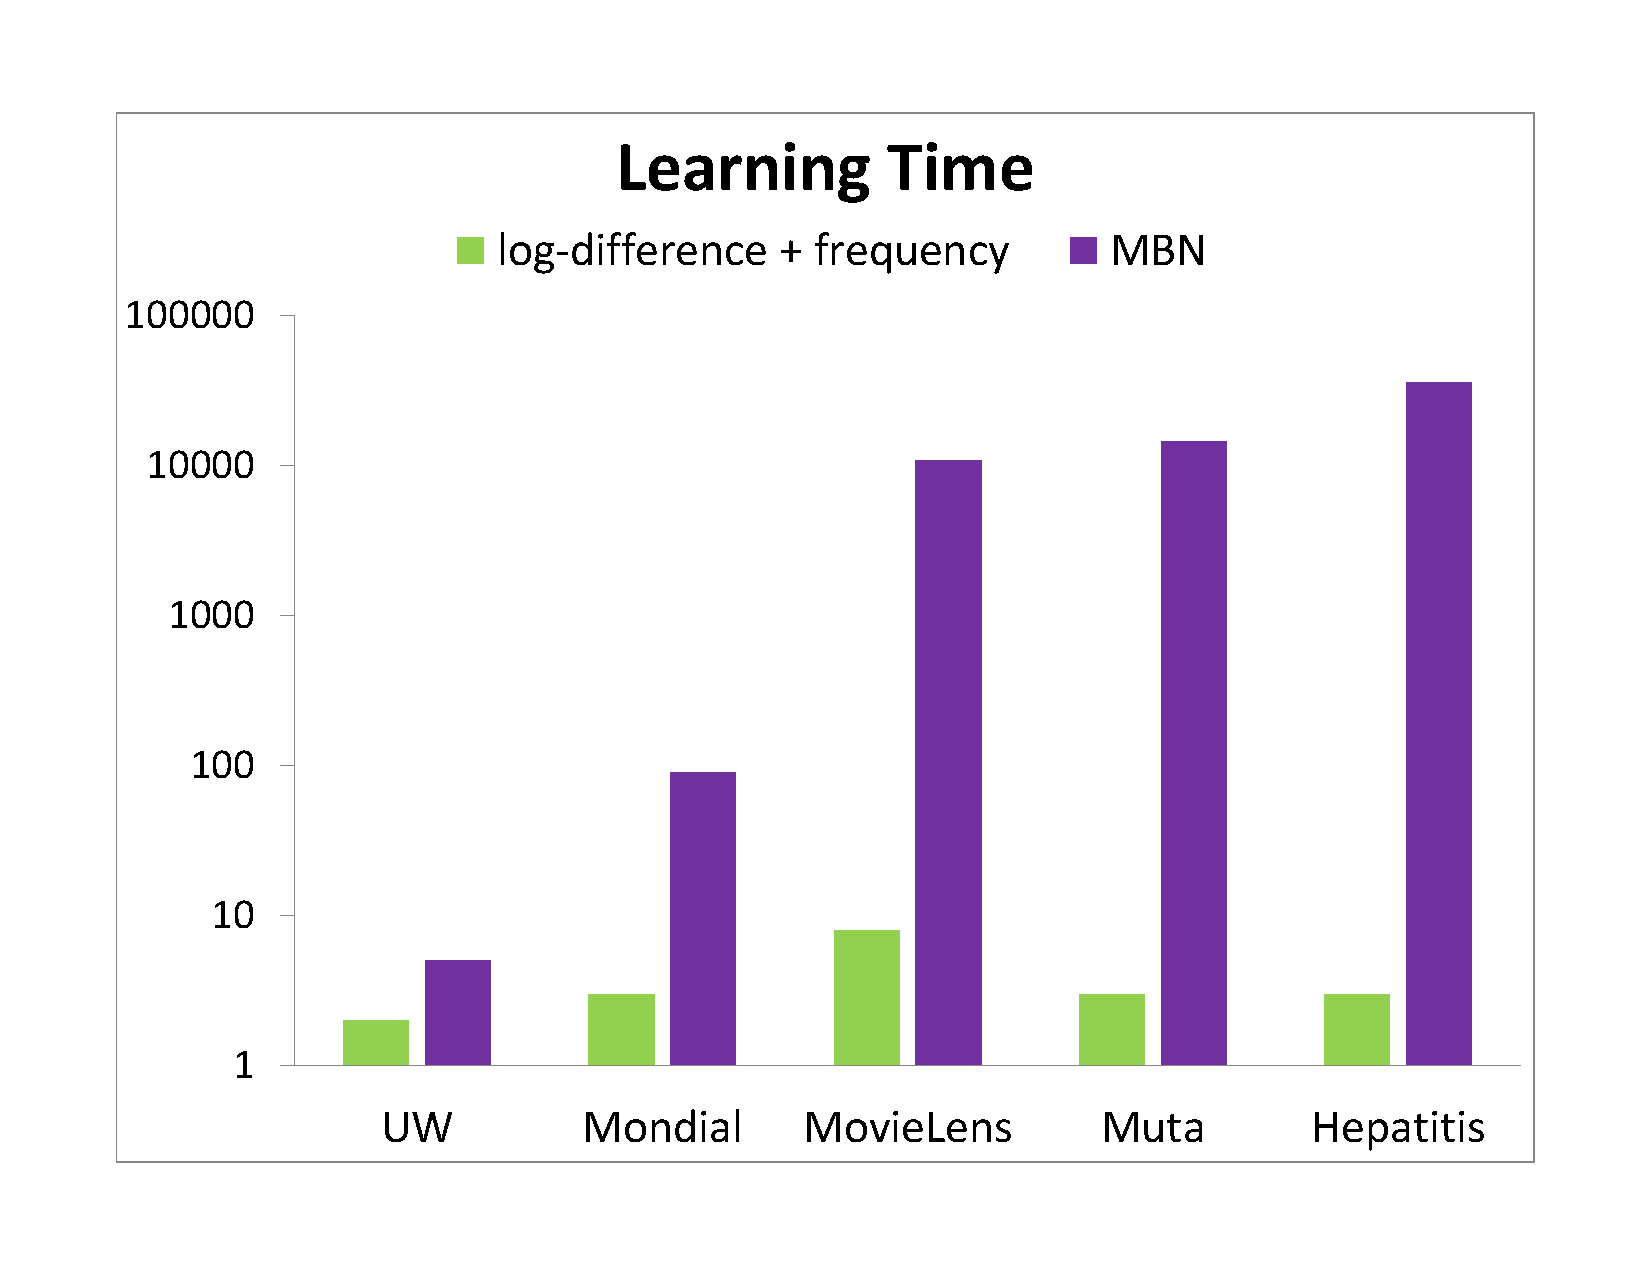
\includegraphics[height=0.5\textheight]{learning_time}
\caption{Predictive Performance averaged over all five benchmark databases. With Bayes net parameters, the frequency model performs better than the count model in terms of likelihood ratios. 
%General weight learning is much slower than Bayes net parameter learning; note that learning times are plotted on a logarithmic scale.
\fixneeded{Expand ``Prob'' to ``Probability''.}
\fixneeded{The 2D bars are much better---but they are still darker at the bottom.}
}
\label{fig:summarize}
\end{center}
\end{figure}

\point{Learning Times}
Table~\ref{table:learn-times} shows run time results for structure and parameter learning. We see \keypoint{clear scalability advantages for the maximum likelihood conditional probability estimates used in the Bayes approach}: they take seconds to compute, whereas Alchemy weight optimization requires as much as 10 hours in the worst case (Hepatitis). 

\begin{table}[t]
\caption{Parameter learning times for MBN and Bayes net methods. 
We characterize each database by its counts of ground atoms, tuples,
and Bayes net parameters, and its time for structure learning. The Bayes net
parameter count is the number of family configurations in the Bayes
net.}
\begin{center}
\begin{tabular}{|l r r c c|r c|}
\hline
Dataset & Literals~ & Tuples~  & Parms. & Struct. & MBN~ & Bayes \\
& ($\times 1000$) & ($\times 1000$) & ($\times 10$) & (s) & {(s)\quad} & (s) \\\hline
UW & {3\quad} & {1\quad} & 12 & 36 & 5~~ & \bf{2} \\
Mondial & {2\quad} & {1\quad}  & 58 & 12 & 90~~ & \bf{3}\\
MovieLens & {170\quad} & {82\quad} & 33 & 72 & 10800~~ & \bf{8}\\
Mutagenesis & {35\quad} & {15\quad} & 88 & 30 & 14400~~ & \bf{3}\\
Hepatitis & {71\quad} & {15\quad} & 79 & 24 & 36000~~ & \bf{3}\\\hline
\end{tabular}
\end{center}
\label{table:learn-times}
\end{table}



\subsection{Evidence for Scaling} \label{sec:weights}
The boxplots in Figure~\ref{fig:boxplots} compare the spread of the weights learned by Alchemy and the corresponding spreads for the log-CP and log-difference methods.
The plots separate {\em 1-variable formulas} that contain only one population variable %(e.g., $\it{gender}(\A) = W,\it{coffee\_dr}(\A) = \true$) 
from {\em 2-variable formulas} that contain more than one population variable.
%(e.g., $\it{gender}(\A) = W,\it{gender}(\B) = W, \it{Friend}(\A,\B) = \true$). 
The 1-variable formulas have just one grounding for a given target node, whereas 2-variable formulas have many. If the computed weights include a scaling component, we expect that the absolute size of weights will be smaller for 2-variable formulas.

\begin{figure}[htbp]
%\vspace{-1cm}
\begin{center}
%\resizebox{0.5\textwidth}{!}{
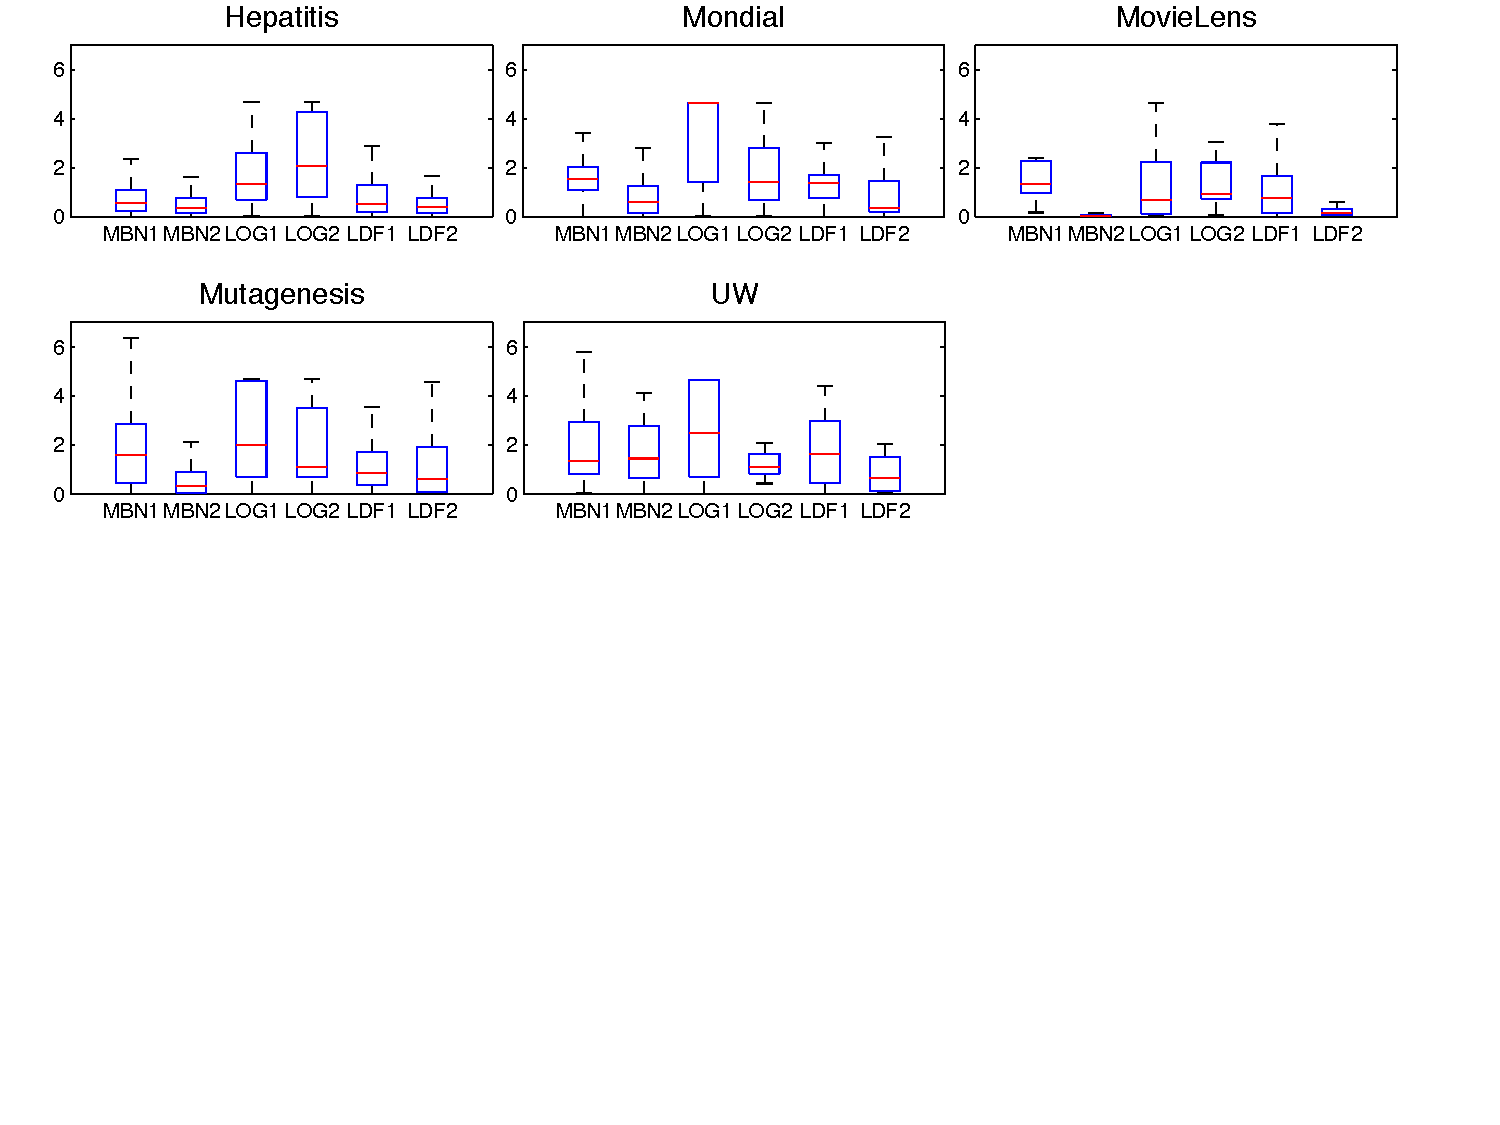
\includegraphics[width=1\textwidth]{boxplots}
%}
\caption{The absolute magnitudes of weights learned from five databases using three estimators for two sizes of formula. MBN=Moralized Bayes Nets, LOG=log(cp), LDF = log-diff. The suffix of 1 or 2 indicates the number of population variables in the formulas. Whiskers represent the 95th percentile.}
\label{fig:boxplots}
\end{center}
\end{figure}

The optimized MBN-weights show clear scaling effects on five databases, with the biggest effect in the MovieLens weights. This is also the dataset where the Bayes net frequency model outperforms
the count model the most on the CLL metric (Table~\ref{table:bn}). Overall, {\em the observed weight magnitudes provide evidence that optimal weights are scaled to balance the diverging instantiation counts for different features.} 

The log-difference weights also show scaling effects on four of the databases, with the largest effect again occuring for MovieLens. This confirms our expectation that information from related entities is less important, although the scaling effect is not as great as with the optimized MBN weights. 
%Therefore, simply using log-difference weights with the count equation is not sufficient for good predictive performance: we need to include a stronger scaling component by (i) transforming the counts to frequencies, or (ii) using (much slower) optimization methods to learn weights.

\point{Summary} 
The findings from this section and the previous one support our claim that balancing the scales of feature functions is important for using Bayes net parameters in a log-linear model. The combination of  transformed BN parameters +feature frequencies  is as predictively accurate as using feature counts with optimized general weights.
While the Bayes net log-linear model is comparable in accuracy, its parameters can be learned much faster than general log-linear weight learning.
%

 
 


\section{Random Selection Inference} \label{sec:random}


The experimental results in the previous two sections indicate that the log-difference frequency equation achieves good predictive accuracy, in addition to scalability and interpretability. In this section, we extend our theoretical understanding of the Bayes net freuquency equations by providing a different deriviations of this method. 

The standard BN product formula defines a joint distribution over template nodes. Recall that the Gibbs conditional probability for this joint distribution is given by the log-linear equation~\ref{eq:bn-mb}. 
In this section we show that frequency regression can be interpreted as the expected value of Equation~\ref{eq:bn-mb}, over {\em random} groundings of the template Bayes net. This value can be computed as follows for a given template Bayes net $\BN$ and query.

\begin{enumerate}
\item Choose a random grounding $\grounding'$ of all population variables in $\BN$. The grounding $\grounding'$ must be consistent with the target node grounding $\grounding$. A random grounding selects a constant for each population variable independently and uniformly.
\item Apply the random grounding to obtain a fully ground Bayes net $\BN_{\grounding'}$. The query conjunction defines a unique value for each node in $\BN_{\grounding'}$. Apply the standard Bayes net equation~\ref{eq:bn-mb} to compute a log-linear score for the query in the single ground BN.
\item Return the average log-linear score over all groundings $\grounding'$.
\end{enumerate}

We need to refine this basic idea to eliminate irrelevant features, i.e., parent-child configurations. A simple way to do this is to consider only groundings such that all features defined by the grounding are relevant.
Algorithm~\ref{alg:random-ground} provides pseudo-code for this computation. Table~\ref{table:random-regress} provides a sample computation of a random selection value for predicting the gender of $sam$ given the database instance of Figure~\ref{fig:pbn}.


\begin{algorithm}[htbp]

%\linesnumbered
\SetKwData{Calls}{Calls}
\SetKwData{Notation}{Notation}
\KwIn{Template Bayes Net $\BN$; Query $\Gprob{\FG{\Ground{\TI}} = \TV} {\QC} = ?$}
\KwOut{Average log-linear score for a random grounding of the template BN.}
\begin{algorithmic}[1]
\STATE Let $\A_{1},\ldots,\A_{a}$ be the population variables in $\Ground{\BN}$.
\FORALL{groundings $\grounding'$ of $\A_{1},\ldots,\A_{a}$, such that $\grounding'$ extends the query grounding $\grounding$}
\FORALL{nodes $\UT$} 
\STATE Let ($\UT = \UV_{\grounding'}$, $\Pa{\UT} = \GroundPrange{U}$) be the family configuration assigned by the query conjunction to the nodes $\UT,\Pa{\UT}$ after applying the grounding $\grounding'$.
\ENDFOR
\IF[$\grounding'$ is relevant]{for all $\UT \in \{\TT\} \cup \Ch{\TT}$, the family configuration ($\UT = \UV_{\grounding'}$,$\Pa{\UT} = \GroundPrange{U}$) is relevant}

% Following statement produces incorrect \vec{u}
%\STATE $\it{score}_{\grounding'} := \sum_{\UT \in \{\TT\} \cup \Ch{\TT}} \ln\cprob{\UT = \UV_{\grounding'}}{\Pa{\UT} = \GroundPrange{U}}$

% Following two statements produce correct \vec{u}
%\STATE $\it{score}_{\grounding'} := \sum_{\UT \in \{\TT\} \cup \Ch{\TT}} \ln$
%\COMMENT {$\cprob{\UT = \UV_{\grounding'}}{\Pa{\UT} = \GroundPrange{U}}$}

% Following statement produces correct \vec{u} (Note that Math mode is now split in two)
\STATE $\it{score}_{\grounding'} := \sum_{\UT \in \{\TT\} \cup \Ch{\TT}} \ln$ $\cprob{\UT = \UV_{\grounding'}}{\Pa{\UT} = \GroundPrange{U}}$
\COMMENT{see Equation~\ref{eq:bn-mb}}
\ENDIF
\ENDFOR
\STATE \Return The average of the relevant scores $\it{score}_{\grounding'}$.
\end{algorithmic}
\caption{Computation for Random Selection Inference.}
\label{alg:random-ground}
\end{algorithm}




\begin{table}
\vspace{-1cm}
\begin{center}
\begin{tabular}{c|l}
Feature \#&Family Configuration\\\hline
1 &$g(sam) = W$,$g(B) = W$, $F(sam,B) = T)$  \\
2 & $g(sam) = W$,$g(B) = \Man$, $F(sam,B) = T)$\\
 3 & $cd(sam) = T,g(sam)=\Woman$ \\\hline
\end{tabular}
\end{center}



\begin{tabular}{c|cc|cc|c}
Grounding & Child = $g(B)$  & CP1 & Child = $cd(sam)$ & CP2 &ln(CP1)+ln(CP2) \\\hline
y1 & Feature 1&0.55 & Feature 3  & 0.80 & -0.82 \\
... & ... & ... & ... & ... \\
y40 & Feature 1 & 0.55& Feature 3  & 0.80 & -0.82 \\
y41 & Feature 2& 0.37 & Feature 3  & 0.80 & -1.22 \\
... & ... & ... & ... & ... \\
y100 & Feature 2 & 0.37& Feature 3 & 0.80 & -1.22 \\
 &  &  &  & Average & -1.06 \\
\end{tabular}
\caption{Computing the random regression for target node value $\it{gender}(sam) = \Woman$. CP = conditional probability. The first 40 rows show the log-linear features for applying the nonrelational Bayes net regression equation~\ref{eq:bn-mb} when the population variable $\B$ is instantiated with one of $sam$'s female friends (cf. Table~\ref{table:log-diff-example}). The next 60 rows show the log-linear factors for instantiating the population variable $\B$ with one of $sam$'s male friends. The random regression result is the average over all the instantiations. Note that the random regression result -1.06 is exactly the same as the result for frequency regression (Table~\ref{table:equation-examples}, row 2, column 1). }
\label{table:random-regress}
\end{table}


Notice that the frequency equations and random selection inference lead to exactly the same value. The next theorem provides a general proof for \keypoint{the  equivalence between frequency and random selection inference}.
 %holds whenever all features are relevant}. 
The general reason for the equivalence is this: Observe that the log-cp frequency equation is a sum of expected values, while the random selection value is the expected value of a sum. As is well known, the sum of expected values of random variables equals the expected value of their sum.

\begin{theorem} \label{th:random-regress} Suppose that all child-parent configurations of the target node are relevant. Then the Gibbs conditional probabilities defined by the following are equal:

\begin{enumerate}
\item Log-difference frequency regression. 
\item Frequency Regression.
\item Random regression.
\end{enumerate}


\end{theorem}

\begin{proof} See the Appendix. %~\ref{app:proofs} for a formal proof.
\end{proof}

\point{Discussion}
%While random regression sums over all groundings of the Markov blanket, the regression equations sum over the {\em non-ground} functor nodes in the Markov blanket. Thus the equations  provide an efficient closed-form for computing the random regression value.
We remark that the above equivalence holds for any graphical model based on a template of logical terms, not only Bayes nets. As Table~\ref{table:random-regress} illustrates, the equivalence can hold even when some features are irrelevant (e.g., the gender of persons who are not friends with Sam). It suffices for random selection inference to be equivalent to the frequency equation if for each family configuration, the expected value of its log-linear score, with respect to groundings of the family nodes only, equals the expected value of its log-linear score with respect to groundings of {\em all} Bayes net nodes. This is guaranteed if for the population variables that are not ground by the query, the set that appears in the parents of the target node is disjoint from the set that appears in the children and spouses of the target node. In our running example, the disjointness condition holds since the only child of the target node is $\it{CoffeeDr}(\A)$ and $\A$ is ground by the query (i.e., $\A \gndlink sam$). Another sufficient condition for the equivalence is that the relevant family configurations can be defined by a uniform condition for the children and parents of the target node, such as $\it{Friend}(\A,\B) = \true$, which is also true in our running example. The close correspondence between random selection inference and the frequency equations completes our argument in support of the frequency log-linear equations. 

We discussed key differences between our approach and KBMC template semantics in Section~\ref{sec:kbmc}. The next section provides further details about relevant related work in statistical-relational learning. 







\section{Related Work} \label{sec:related} We first discuss work on directed graphical  models for relational data, then consider other graphical model classes such as Markov and dependency networks. \cite{Heckerman2000} {\em et al.} compare Bayes, Markov and dependency nets in detail for nonrelational data. 

\paragraph{Directed Graphical Models} There are several proposals for defining directed relational template models, based on graphs with directed edges or rules in clausal format \cite{Kersting2007,Getoor2007c,Fierens2009,Milch2007}. While the template model need not be a Bayes net (in contrast with our Template Bayes nets), the usual application of KBMC semantics requires that the instantiated model should be a Bayes net (cf. Section~\ref{sec:kbmc}). 
In order to define the probability of a child node conditional on multiple instantiations of a parent set, template semantics for directed models therefore requires the addition of combining rules \cite{Kersting2007} or aggregation functions (usually with extra parameters) \cite{Getoor2007c}. As described by \cite{Kersting2007}, aggregate functions can be added to a Template Bayes net by including functor nodes with aggregates (e.g., $\it{AvgGrade}(\S)$ may represent the average grade of a student). Combining rules such as the arithmetic mean~\cite{Natarajan2010} combine global parameters with a local scaling factor, as does our log-linear model. 
Our frequency model is similar to a combining rule using the {\em geometric mean} rather than the arithmetic mean, with
the important difference 
that the geometric mean is applied to the entire Markov blanket of the target node, whereas usually a combining rule applies only to the parents of the target node. To our knowledge, the geometric mean has not been used with ground Bayes nets before.

\paragraph{Markov Networks} Relational log-linear models
are usually associated with undirected graphs~\cite{Sutton2007}, such as Relational Markov networks \cite{Taskar2002} and Markov Logic Networks \cite{Domingos2009}. To our knowledge, this is the first paper that specifies a log-linear model for Bayes nets directly. Several researchers have examined converting a Bayes net relational model to a Markov net. Since Markov nets define a log-linear inference model, this conversion strategy entails using a log-linear model for Bayes nets. 
Richardson and Domingos propose converting a Bayes net to a Markov Logic network using moralization, with log-conditional probabilities as weights \cite{Domingos2007}. 
This is also the standard Bayes net conversion recommended by the Alchemy system \cite{bib:bayes-convert}. 
The moralization method inferences are equivalent to our equation log(cp)+ count. 
To our knowledge, our experiments are the first that evaluate the log(cp)+count equation, and our three comparison equations are novel. Natarajan et al. \cite{Natarajan2010} consider moralization with Bayes nets that have been augmented with combining rules.
We consider tabular Bayes nets whose parameters are CP-table entries only. 
Combining rules do not generally lead to log-linear models. 
 
\paragraph{Dependency Networks} Dependency networks are directed graphical models that allow cycles \cite{Heckerman2000}. For instance, the ground BN of Figure~\ref{fig:recurse-bn}(bottom) is a valid dependency net structure. Relational Dependency networks (RDNs)~\cite{Neville2007} have been an influential recent development because they can accommodate the cyclic dependencies that are common in relational data. The parameter space of dependency networks comprises the set of Gibbs conditional probabilities. The RDN solution to the cyclicity problem is therefore the same as what we propose in this paper: define local Gibbs probability distributions rather than a single acyclic global model. The original RDN work used aggregate functions to combine different instantiations of a target node's Markov blanket. Learning dependency networks with log-linear relational models was investigated by Khot {\em et al.} \cite{Khot2011}; this work used feature counts, not frequencies. In this paper, we do not learn Gibbs conditional distributions directly. Instead, we apply previous algorithms
to learn a BN structure, and derive Gibbs probabilities from the learned structure and maximum (pseudo)-likelihood estimates of the BN parameters.

In sum, while log-linear models for Gibbs probabilities have been investigated for other graphical model classes, ours is the first multi-relational model of this type for Bayes nets. Our use of frequencies vs. counts for feature functions is new. 


\section{Conclusion and Future Work} 
\label{sec:conclusion}

This paper presented a new log-linear inference equation for applying Bayes nets to relational data. For a fixed template Bayes net, the equation defines the Gibbs conditional probability of a target node given an assignment of values to all other nodes. A log-linear model is defined by: a set of features, and for each feature, a feature function and a feature weight. The predicted conditional probability is the exponentiated weighted sum of feature function values. In our proposed model, the features are all family configurations in for a family in the Bayes net, whose child node is either the target node or a child of the target node. The weight associated with a child-parent feature is computed as the log-difference of two quantities determined by the BN parameters: (i) the conditional probability of the child value, given its parent configuration, and (ii) the marginal probability of the child value. The feature function is the frequency with which the feature is instantiated in the given query, normalized with respect to relevant features only. 

Our experiments on five benchmark datasets compared our log-difference frequency equation to several alternatives: using counts as feature frequencies, and  using log-conditional probabilities as feature weights. We also compared using transformed Bayes net parameters as weights to using weights directly learned from the data by log-linear optimization methods. Our frequency equation achieved the best predictive performance on all but one dataset. Using the maximum likelihood values as Bayes net parameters is much faster than optimizing weights using standard log-linear methods (Markov Logic), typically seconds vs. hours. 
%The impact of using Bayes net structures was compared to structure learning with the state-of-the-art MLN-Boost method. Bayes net learning was much faster than the boosting approach, with competitive predictive accuracy.

Different model classes each have their advantages and disadvantages. Nonetheless  the combination of Bayes nets and  our proposed log-linear model,  offers a unique set of advantages compared to other inference methods for multi-relational data, in terms of the  \emph{interpretability} and \emph{scalability} of both structure and parameter learning: Feature weights are readily interpreted as a log-transformation of the Bayes net conditional probability parameters, and the Bayes net parameters can be computed in closed-form as the empirical frequencies. 

We have established novel connections between the use of frequency feature functions and what, at first sight, appear to be unrelated issues such as the imbalance problem, pruning irrelevant features, maximum likelihood estimation, and the random selection interpretation of template Bayes nets. (1) The imbalance problem arises because feature instantiation counts in relational data can diverge by orders of magnitude. Rescaling counts as frequencies produces feature function values on the same scale. According to our experiments, changing the feature function is a more effective approach to the imbalance problem than using the weight parameters to rescale (assign smaller weight magnitudes to larger feature counts). (2) It is important not only to prune irrelevant features, but also to define instantiation frequencies over the space of relevant features only. (3) Maximum likelihood estimation is competive with optimizing weight parameters from the data only when relevant feature frequencies are used as feature functions. (4) Under mild assumptions, our frequency equation is equivalent to a {\em random selection} method, where the prediction score for a target node value is defined as the expected score, with respect to a random instantiation of the template Bayes net, computed using the standard Bayes net equation for a Gibbs conditional probability.

There are several avenues for future work. While we focus on Bayes nets, the imbalance problem arises also for other relational models. Our solution of changing the predictor space from counts to frequencies applies to log-linear models in general.
\cite{Sutton2007,Taskar2002,Domingos2009}.
The frequency equation can be combined with other log-linear learning methods, for example within a model ensemble. Functional gradient boosting \cite{Khot2011} is a powerful technique for learning such ensembles. 

Our model introduces a 1-1 correspondence between log-linear weights and Bayes net parameters. Therefore log-linear regularization techniques \cite{Huynh2008} can be used for smoothing parameter estimates in template Bayes nets, and for detecting irrelevant features. 

Local Gibbs probability models  may be inconsistent in the sense that there is no joint distribution that agrees with the local conditional probabilities \cite{Heckerman2000}. An open theoretical question is whether our local frequency equations for different target nodes are guaranteed to be mutually consistent. If they are inconsistent, a possible approach is to apply the recent averaging methods for dependency networks \cite{Lowd2012,Poole2013}.

Our log-linear equation with relevant feature frequencies appears to be a principled, fast-to-learn, and accurate model for relational prediction with Bayes nets.




\section*{Acknowledgements} This work was supported by Discovery Grants to Oliver Schulte from the Natural Science and Engineering Council of Canada. Zhensong Qian was supported by a grant from the China Scholarship Council. A preliminary versions of this paper was presented at the StarAI 2012 workshop. We are indebted to workshop reviewers and participants for helpful comments.

\section*{Appendix: Proofs} \label{app:proofs}

Our two theorems concern the frequency regression equation, where the predictors are relevant frequencies and the weights are log-conditional probabilities. The formal definition of the \defterm{log-cp frequency equation} is



\begin{eqnarray} 
  \Gprob{\FG{\Ground{\TI}} = \TV} {\QC} \propto  \exp  \sum_{\UT} \sum_{\UV,\Prange{\UT}}   \ln \cprob{\UT = \UV}{\Pa{\UT} = \Prange{\UT}}      \cdot 
    \Relfreq{\Appendterm{\Ground{\UI}  = \UV} {\Ground{\Pa{\UI}} = \Prange{\UT}}} {\Qconj} \label{eq:frequency}.
\end{eqnarray}



\begin{proposition}
Frequency regression returns the same result when used with log-cp weights and when used with log-difference weights.
\end{proposition}

\begin{proof} Our approach is to show that the log-difference equation can be factored such that (i) the bias weight is cancelled out,  and (ii) the difference between the result and the frequency equation is a constant factor that is independent of the target node value. Thus the normalized probability defined by each equation is the same.

We begin with some observations about the independence of relevant counts from the target node value. The first observation is that for a node that is not the target node, \keypoint {the relevant count of any of its family configurations is independent of the target node value}:

\newcommand{\Qconjnew}{\Appendterm{\FG{\Ground{\TI}} = \TV'} {\DB}}

\begin{equation} \label{eq:independent-family}
 \Relcount{\Appendterm{\Ground{\UI}  = \UV} {\Ground{\Pa{\UI}} = \Prange{\UT}}} {\Qconj} =
 \Relcount{\Appendterm{\Ground{\UI}  = \UV} {\Ground{\Pa{\UI}} = \Prange{\UT}}} {\Qconjnew}
\end{equation}

\noindent for any target node values $\TV$ resp. $\TV'$. The reason for the independence is that a true family grounding with $\TV$ can be changed to a true family grounding where the only change is that the target node is assigned value $\TV'$ rather than $\TV$. 
%\this assumes that no other parent has the same functor as the target node}  

If the target node is the child in the family configuration, the relevant count is, for the same reason, independent of the target node value, as long as the child node value is consistent with the target node value

\begin{equation} \label{eq:independent-target-child}
 \Relcount{\Appendterm{\FG{\Ground{\TI}} = \TV} {\Pa{\Ground{\TI}} = \Prange{\TT}}} {\Qconj} =
 \Relcount{\Appendterm{\FG{\Ground{\TI}} = \TV'} {\Pa{\Ground{\TI}} = \Prange{\TT}}} {\Qconjnew}
\end{equation}

\noindent for any target node values $\TV$ resp. $\TV'$. If the assignment to the child node is inconsistent with the target node value, the number of true instantiations is 0:

\begin{equation} \label{eq:inconsistent}
 \Relcount{\Appendterm{\FG{\Ground{\TI}} = \TV} {\Pa{\Ground{\TI}} = \Prange{\TT}}} {\Qconjnew} =
 0
\end{equation}
whenever $\TV \neq \TV'$. 
%
The \defterm{marginal frequency} of a child node value is obtained by summing over the frequencies of family configurations with that child node value:

\begin{equation*} 
 \Relfreq{\Ground{\UI}  = \UV} {\Qconj} \equiv \sum_{\Prange{\UT}}\Relfreq{\Appendterm{\Ground{\UI}  = \UV} {\Ground{\Pa{\UI}} =\Prange{\UT}}} {\Qconj}
\end{equation*}
%whenever $\TV \neq \TV'$. 
%
For the special case in which the target node is the child in the family, all consistent family configurations agree with the target node value, which therefore has marginal frequency 1. In other words, Equation~\eqref{eq:inconsistent} implies that 

\begin{equation} \label{eq:prob1}
\Relfreq{\FG{\Ground{\TI}} = \TV} {\Qconj} = 1.
\end{equation}

From Equation~\eqref{eq:prob1} and the definition of marginal frequency we have the equalities

\begin{eqnarray}
\sum_{\UT} \sum_{\UV} \sum_{\Prange{\UT}} \ln \jprob{\UT = \UV} \cdot \Relfreq{\Appendterm{\Ground{\UI}  = \UV} {\Ground{\Pa{\UI}} = \Prange{\UT}}} {\Qconj} \nonumber\\
=\sum_{\UT} \sum_{\UV} \ln \jprob{\UT = \UV} \sum_{\Prange{\UT}} \nonumber\Relfreq{\Appendterm{\Ground{\UI}  = \UV} {\Ground{\Pa{\UI}} = \Prange{\UT}}} {\Qconj}
\\ = \ln \jprob{\TT = \TV} \cdot 1 + \sum_{\UT \neq \TT} \sum_{\UV} \ln \jprob{\UT = \UV} \cdot \Relfreq{\Ground{\UI}  = \UV} {\Qconj} \label{eq:factorout}
\end{eqnarray}


We next factor the log-difference equation by multiplying out the log-difference. To simplify the expressions, we work with the linear sum inside the $\exp$ expression.



\begin{eqnarray*}
 \ln \jprob{\TT = \TV} + \sum_{\UT} \sum_{\UV,\Prange{\UT}}  
 \left[ \ln \cprob{\UT = \UV}{\Pa{\UT} = \Prange{\UT}} - \ln \jprob{\UT = \UV} \right] 
    \cdot 
\Relfreq{\Appendterm{\Ground{\UI}  = \UV} {\Ground{\Pa{\UI}} = \Prange{\UT}}} {\Qconj}  
 \\
 =  
 \ln \jprob{\TT = \TV}  + \sum_{\UT} \sum_{\UV,\Prange{\UT}} \ln \cprob{\UT = \UV}{\Pa{\UT} = \Prange{\UT}} +\Relfreq{\Appendterm{\Ground{\UI}  = \UV} {\Ground{\Pa{\UI}} = \Prange{\UT}}} {\Qconj} \\
 - \sum_{\UT} \sum_{\UV,\Prange{\UT}} \ln \jprob{\UT = \UV} \cdot \Relfreq{\Appendterm{\Ground{\UI}  = \UV} {\Ground{\Pa{\UI}} = \Prange{\UT}}} {\Qconj} \\
=  \ln \jprob{\TT = \TV}  + \sum_{\UT} \sum_{\UV,\Prange{\UT}} \ln \cprob{\UT = \UV}{\Pa{\UT} = \Prange{\UT}} \cdot  \Relfreq{\Appendterm{\Ground{\UI}  = \UV} {\Ground{\Pa{\UI}} = \Prange{\UT}}} {\Qconj}  \\
- \ln \jprob{\TT = \TV}) - \sum_{\UT \neq \TT} \sum_{\UV} \ln \jprob{\UT = \UV} \cdot \Relfreq{\Ground{\UI}  = \UV} {\Qconj} \\
=  \sum_{\UT} \sum_{\UV,\Prange{\UT}} \ln \cprob{\UT = \UV}{\Pa{\UT} = \Prange{\UT}} \cdot  \Relfreq{\Appendterm{\Ground{\UI}  = \UV} {\Ground{\Pa{\UI}} = \Prange{\UT}}} {\Qconj}  \\
 - \sum_{\UT \neq \TT} \sum_{\UV} \ln \jprob{\UT = \UV} \cdot \Relfreq{\Ground{\UI}  = \UV} {\Qconj} 
\end{eqnarray*}

The last step follows by cancelling out the marginal log-probabilities $\ln \jprob{\TT = \TV}$. The last-but-one-step follows from Equation~\eqref{eq:factorout}. Comparing the exponential of the last line and the log-cp frequency equation~\eqref{eq:frequency}, we see that the only difference between the log-difference and the log-cp frequency equation is the factor $$ \exp \left( - \sum_{\UT \neq \TT} \sum_{\UV} \ln \jprob{\UT = \UV} \cdot \Relfreq{\Ground{\UI}  = \UV} {\Qconj} \right).$$ Clearly the marginal probability $\jprob{\UT = \UV}$ does not depend on the target node value when $\UT \neq \TT$. Also, Equation~\eqref{eq:independent-family} implies that the relevant family configuration counts do not depend on the target node value. Therefore neither do the relevant family configuration frequencies. Hence the displayed term is independent of the target node value. This means that the log-cp and log-difference frequency regression equations differ only by a factor that is independent of the target node value. Therefore they agree on the prediction for the normalized probability of the target node value.


\end{proof}



\begin{theorem}
Suppose that all child-parent configurations of the target node are relevant.  Then the frequency regression value  for a target node (Equation~\eqref{eq:frequency}) equals the random regression value. 
\end{theorem}

%\begin{theorem} \label{prop:randomize}
%The frequency regression value  for a target node (Equation~\eqref{eq:frequency}) equals the random regression value. 
%%; in symbols, $P^{r} = P^{\pseudo}$.
%\end{theorem}
%

\begin{proof} Let $\BN$ be the partially ground template model that results from applying the target grounding. We write $\groundall$ for the set of all groundings of {\em all} population variables in the partially ground graph $\BN$.
\newcommand{\BigCvar}{\mathrm{N}}
\newcommand{\BigCount}[2]{\BigCvar\left[#1;#2\right]}
For each partially ground family formula $\Appendterm{\Ground{\UI}  = \UV} {\Ground{\Pa{\UI}} = \Prange{\UT}}$, let $$\BigCount{\Appendterm{\Ground{\UI}  = \UV} {\Ground{\Pa{\UI}} = \Prange{\UT}}} {\QC,\Ground{\TI} = \TV}$$ be the number of simultaneous groundings of {\em all} variables in $\BN$ that satisfy $\Appendterm{\Ground{\UI}  = \UV} {\Ground{\Pa{\UI}} = \Prange{\UT}}$. 
Consider a family formula $(\Appendterm{\Ground{\UI}  = \UV} {\Ground{\Pa{\UI}} = \Prange{\UT}})$ whose child is the target node or one of its children. For each simultaneous grounding $\grounding \in \groundall$ that satisfies the family formula  in the query conjunction, the associated factor $\ln \cprob{\UT = \UV}{\Pa{\UT} = \Prange{\UT}}$ appears once in the logarithm of the non-relational Gibbs probability equation~\ref{eq:bn-mb}. Therefore  random regression is equivalent to the formulas

\begin{eqnarray} 
\Gprob{\FG{\Ground{\TI}} = \TV} {\QC} \propto \nonumber \\\exp (\frac{1}{|\groundall|} \sum_{\UT} \sum_{\UV,\Prange{\UT}} \ln \cprob{\UT = \UV}{\Pa{\UT} = \Prange{\UT}} \cdot \BigCount{\Appendterm{\Ground{\UI}  = \UV} {\Ground{\Pa{\UI}} = \Prange{\UT}}} {\QC,\Ground{\TI} = \TV}) \label{eq:simplify-halpern}\\
= \exp (\sum_{\UT} \sum_{\UV,\Prange{\UT}}  \ln \cprob{\UT = \UV}{\Pa{\UT} = \Prange{\UT}} \cdot \frac{\BigCount{\Appendterm{\Ground{\UI}  = \UV} {\Ground{\Pa{\UI}} = \Prange{\UT}}} {\QC,\Ground{\TI} = \TV}}{|\groundall|})   \nonumber
\end{eqnarray}
where the sum ranges over family configurations of the target node and its children as usual. To establish the equivalence of Equation~\eqref{eq:simplify-halpern} with the log-cp frequency equation~\eqref{eq:frequency}, it suffices to show that the count fraction in the last random regression equality is another way of computing the frequency of a family configuration. In symbols, we show that

\begin{equation} \label{eq:prob}
\Freq{\Appendterm{\Ground{\UI}  = \UV} {\Ground{\Pa{\UI}} = \Prange{\UT}}} {\QC,\Ground{\TI} = \TV} 
= \frac{\BigCount{\Appendterm{\Ground{\UI}  = \UV} {\Ground{\Pa{\UI}} = \Prange{\UT}}} {\QC,\Ground{\TI} = \TV}}{|\groundall|}
\end{equation}

The equivalence with relevant frequency regression follows from the theorem's premise that the relevant frequency $\Relfreq{}{}$ and the unqualified frequency $\Freq{}{}$ are the same. 
%
%We now show the equivalence of Equation~\eqref{eq:simplify-halpern} to the frequency regression equation~\eqref{eq:frequency}. The key is to observe that the frequency of a family configuration can be computed in two equivalent ways. The first is used in frequency regression, the second is used (implicitly) in random regression.
%[Oliver: rewrite using random regression first]

We introduce some notation to establish Equation~\ref{eq:prob}, which says that the frequency of a family configuration can be computed in terms of groundings for all variables in the Bayes net. The basic reason why this is true is that, compared to  groundings for variables in the family only, the number of possible groundings for the family  increases by a constant factor that cancels out when we divide by the total number of possible groundings $|\groundall|$. 
Write $m_{\Ground{\UI}}$ for the number of possible groundings of the population variables that occur in the family of child node $\Ground{\UI}$.
Write $\bar{m}_{\Ground{\UI}}$ for the number of possible groundings of the population variables that do {\em not} occur in the family of child node $\Ground{\UI}$. For instance, if variables $\A_{1},\A_{2}$ occur in the family of $\Ground{\UI}$, and variable $\A_{3}$ does not, then $m_{\Ground{\UI}} = |\population_{\A_{1}}| \cdots |\population_{\A_{2}}|$, and $\bar{m}_{\Ground{\UI}} = |\population_{\A_{3}}|$ where $\population_{\A_{i}}$ is the population associated with variable $\A_{i}$.  Then we have
\begin{eqnarray*}
|\groundall| & = & m_{\Ground{\UI}} \cdot \bar{m}_{\Ground{\UI}}\\
\BigCount{\Appendterm{\Ground{\UI}  = \UV} {\Ground{\Pa{\UI}} = \Prange{\UT}}} {\QC,\Ground{\TI} = \TV} & = & \Count{\Appendterm{\Ground{\UI}  = \UV} {\Ground{\Pa{\UI}} = \Prange{\UT}}} {\QC,\Ground{\TI} = \TV}\cdot \bar{m}_{\Ground{\UI}}\\
\frac{\BigCount{\Appendterm{\Ground{\UI}  = \UV} {\Ground{\Pa{\UI}} = \Prange{\UT}}} {\QC,\Ground{\TI} = \TV}}{|\groundall|} &=&\frac{\Count{\Appendterm{\Ground{\UI}  = \UV} {\Ground{\Pa{\UI}} = \Prange{\UT}}} {\QC,\Ground{\TI} = \TV}}{m_{\Ground{\UI}}}\\
 =  \Freq{\Appendterm{\Ground{\UI}  = \UV} {\Ground{\Pa{\UI}} = \Prange{\UT}}} {\QC,\Ground{\TI} = \TV}
\end{eqnarray*}
The first, second, and fourth equality follow from the definition of the relevant concepts. The third equation follows from the first two after cancelling $ \bar{m}_{\Ground{\UI}}$ from numerator and denominator. The equations entail the alternative expression~\eqref{eq:prob} for the frequency of a family configuration. This suffices to establish the equivalence of the frequency equation~\eqref{eq:frequency} with the random regression formula~\eqref{eq:simplify-halpern}.
\end{proof}


%% The file named.bst is a bibliography style file for BibTeX 0.99c
%\bibliographystyle{plain}
\bibliographystyle{theapa}
\bibliography{master}
\end{document}
